\documentclass[11pt]{article}
\usepackage[T1]{fontenc}
\usepackage[utf8]{inputenc}
\usepackage[margin=1in]{geometry}
\usepackage{amsmath,amssymb,amsthm,mathtools,booktabs,array}
\usepackage{microtype}
\usepackage{tikz}
\usetikzlibrary{positioning}
\usepackage[numbers,sort&compress]{natbib}
\usepackage[colorlinks=true,allcolors=blue]{hyperref}
\hypersetup{pdftitle={Exact Feasibility of Resistive and AC Power Networks}}
\newcommand{\R}{\mathbb{R}}
\newcommand{\Q}{\mathbb{Q}}
\newcommand{\ER}{\exists\mathbb{R}}
\newcommand{\NP}{\mathsf{NP}}
\newcommand{\PSPACE}{\mathsf{PSPACE}}
\newcommand{\RPF}{\textnormal{\textsc{RPF}}}
\newcommand{\ACPF}{\textnormal{\textsc{ACPF}}}
\newcommand{\ETRINV}{\textnormal{\textsc{ETR-INV}}}
\newcommand{\power}{\mathcal{P}}
\newcommand{\comp}[1]{\overline{#1}}
\newtheorem{theorem}{Theorem}[section]
\newtheorem{lemma}[theorem]{Lemma}
\newtheorem{proposition}[theorem]{Proposition}
\newtheorem{corollary}[theorem]{Corollary}
\theoremstyle{definition}
\newtheorem{definition}[theorem]{Definition}
\theoremstyle{remark}
\newtheorem{remark}[theorem]{Remark}

\title{Exact Feasibility of Resistive and AC Power Networks}
\author{}
\date{}
\begin{document}
\maketitle
\begin{abstract}
Exact feasibility of a resistive power network is complete for the existential
theory of the reals, even on connected simple planar bipartite graphs of
maximum degree three, with unit conductance and any prescribed fixed lower
bound on girth.
Positive voltage intervals and signed injection intervals have endpoints in
fixed finite rational sets. A reduction from bounded addition and inversion
preserves the entire solution set by a rational bijection. It transfers to
AC networks with resistive lines and zero reactive injections, or one-sided
reactive intervals of positive width. For rational cosine limits in $(-1,1]$, we encode cycle winding to distinguish consistent real
bus angles from principal line angles; separate completeness results cover
bus-angle boxes and strictly positive principal-angle windows.
The same restricted resistive networks realize every compact semialgebraic
feasible-set topology. Rational equivalence holds precisely for compact basic
closed sets defined over $\Q$, and unique voltages can have arbitrary algebraic
degree. Quantitative residual transfer yields explicit infeasible fixed-data
networks with doubly exponentially small residuals, matching the general
separation scale. Short rational certificates for a specified gap promise and
quantitative reactive stability explain what finite-precision feasibility can
certify. All constructions are supported by reproducible exact-arithmetic
checks.
\end{abstract}
\section{Introduction}
\label{sec:introduction}

Power-flow feasibility asks whether the electrical laws and operating limits
of a network can hold simultaneously. Even without switching decisions,
power is nonlinear in voltage. This leaves two separate questions: how hard
is it to decide exact feasibility, and how much does a small numerical
residual establish? We answer both for a resistive model with rational
conductances, positive voltage intervals, and signed injection intervals,
and transfer the exact classification to several precisely specified AC
models.

Our main result is that exact resistive feasibility is complete for
$\ER$, the class associated with the existential theory of the reals.
For each fixed integer $r$, hardness holds simultaneously on connected
simple planar bipartite graphs of maximum degree three and girth at least
$r$, with unit conductance and interval endpoints from fixed finite rational
sets depending only on $r$ (Theorem~\ref{thm:structural}). Thus neither
large numerical coefficients nor dense graphs are required. The class
satisfies $\NP\subseteq\ER\subseteq\PSPACE$; its relation to exact
real-valued certificates and its range of applications are surveyed by
\citet{SchaeferEtAl2024}. In particular, a polynomial-size certificate scheme
for every feasible instance, with deterministic polynomial-time verification,
would imply $\NP=\ER$.

\subsection{Results and proof strategy}

The construction starts from bounded addition and inversion. A voltage-pinned
bus imposes an affine relation on neighboring voltages. Alternating complement
paths supply distinct copies of a source variable without increasing the
degree beyond three. One small nonlinear gadget enforces inversion. Every
source solution has exactly one network extension, and the original variables
are read directly from designated bus voltages
(Section~\ref{sec:resistive}). A bounded arithmetic crossover gives planarity;
free-injection connectors give connectedness; and harmonic subdivisions give
unit conductance, bipartiteness, and prescribed girth
(Section~\ref{sec:structural}). These transformations preserve the rational
solution-set correspondence. The hard graphs may have many cycles: the girth
statement does not assert hardness on trees.

For AC feasibility, a local cosine inequality constrains the principal angle
of each line but need not provide consistent real bus angles. A cycle can
wind once around the origin while every local inequality holds. We give a
polynomial-size existential-real encoding of the missing cycle condition,
including unequal voltage magnitudes and every rational cosine in $(-1,1]$.
For purely resistive lines, a real-angle energy identity then forces equal
angles when all reactive injections are zero. This transfers the resistive
classification to AC feasibility. The same transfer allows all reactive
intervals to have positive width on a common side of zero. We also treat a
rectangular bus-angle box and principal-angle windows that are strictly
positive and shrink with the number of buses
(Section~\ref{sec:ac}). The latter windows have polynomial-bit rational
cosines; unlike the fixed-data resistive construction, those cosines need
not belong to a fixed finite set.

The solution-set correspondence yields a sharp algebraic statement
(Section~\ref{sec:algebraic}). A compact semialgebraic set defined over
$\Q$ is rationally equivalent to a feasible voltage set if and only if
it is basic closed over $\Q$, meaning that a conjunction of polynomial
equalities and weak inequalities suffices to describe it. Arbitrary compact
semialgebraic sets still occur up to semialgebraic homeomorphism. Distinguishing
these two forms of universality is necessary: rational equivalence preserves
more than topology. In particular, a rational network may have a unique
feasible voltage vector with a designated voltage generating any prescribed
real algebraic number field. Appendix~\ref{app:arithmetic} supplies the
conjunction-only arithmetic construction used for these conclusions.

Finally, Section~\ref{sec:numerical} quantifies the difference between exact
and approximate feasibility. The ordinary reduction has a two-sided residual
bound. An explicit infeasible family of $O(k)$ buses admits states with
residual less than $2^{-2^k}$. A general polynomial-minimum bound gives the
matching doubly exponential separation scale for fixed-data bounded-degree
networks. A small residual therefore cannot serve as a universal exact
feasibility test at polynomial precision. At a specified gap promise,
however, short rational certificates exist. A quantitative energy estimate
also controls angle deviation and active-power error when reactive injections
are small. Appendix~\ref{app:verification} records exact-arithmetic checks
and analytically resolves the examples used in earlier numerical experiments.

\subsection{Relation to previous work and model scope}

The resistive equations are the physical direct-current power-flow model
studied by \citet{GanLow2014}. They are distinct from the linear ``DC
approximation'' of AC power flow. Gan and Low give sufficient conditions for
exactness of a second-order cone relaxation of resistive optimal power flow,
including conditions involving voltage upper bounds and injection lower
bounds. Our classification concerns arbitrary allowed bus intervals and does
not assume those exactness conditions. Both voltage and injection bounds may
be singletons, independently; in particular, a voltage-pinned bus may also
have a prescribed injection. Section~\ref{sec:foundations} makes these input
choices explicit because the reduction uses them.

A different resistive model fixes source voltages and asks which
constant-power demands can be supplied at load buses.
\citet[Theorem 3.22]{JeeningaEtAl2023} characterize both exact feasibility and
its interior by matrix-inequality alternatives, and establish convexity of
the feasible demand set. This is a different feasible set from the one
obtained by placing voltage and injection intervals at every bus type.
Nor does an exact matrix-inequality characterization alone establish a
polynomial-time Turing algorithm for exact feasibility.

For AC networks, \citet{BienstockVerma2019} prove strong NP-hardness in a
lossless model with fixed voltage magnitudes and unconstrained reactive
power. \citet{LehmannEtAl2016} prove NP-hardness on trees, already using star
networks, in a fixed-magnitude model with active and reactive constraints.
These results concern different physical restrictions from our resistive-line
AC subclass, where variable magnitudes implement arithmetic and reactive
balance forces equal angles. Our rational-cosine encoding also states
explicitly how angle limits are represented in a binary input.

The connection between resistive AC networks and zero reactive injections
appears in \citet[Appendix B, Case 2]{LavaeiLow2012}. The reactive equations
are also weighted sine-coupling equilibrium equations, as in the oscillator
framework of \citet{DorflerEtAl2013}. We use a self-contained energy proof
with a consistent real-angle lift. The distinction is essential on meshed
networks: the winding examples in Section~\ref{subsec:principal} satisfy
zero reactive injection with nonconstant phasors.

Approximation results address a further distinction.
\citet[Theorem 7 and Corollary 8 of the arXiv version]{BienstockMunoz2018}
give LP approximation
schemes for polynomial network optimization and bounded-treewidth AC optimal
power flow, with scaled feasibility and optimality tolerances. Their
guarantees do not decide exact feasibility. Our gap-promise certificate
result likewise states its tolerance and promise explicitly; it does not
resolve the unpromised approximate-membership question posed for the
lossless fixed-magnitude model in
\citet[Section 1.3]{BienstockVermaPreprint2019}.

The arithmetic starting problem comes from
\citet{AbrahamsenEtAl2018,AbrahamsenEtAl2022}; its planar crossover comes from
\citet{DobbinsEtAl2023}. For solution-set universality, we develop the
conjunction-only part of the arithmetic method of
\citet{AbrahamsenMiltzow2019}, with explicit gate ranges and a proof of the
basic-closed restriction. Semialgebraic triangulation
\citep{OhmotoShiota2017} supplies the separate topological statement, and
the polynomial-minimum theorem of \citet{JeronimoEtAl2013} supplies the
general residual lower bound. The electrical constructions and their
quantitative properties are proved directly below.

\section{Exact feasibility and the resistive model}
\label{sec:foundations}

In a resistive network, current depends linearly on bus voltages, but power is
the product of voltage and current. This distinction makes exact feasibility a
quadratic problem even when the network has no discrete controls. We study its
complexity with interval restrictions on both voltage and net power injection.
The model concerns direct-current electrical networks; it is distinct from
the linear ``DC approximation'' of an alternating-current network.

\subsection{Input model and complexity convention}

Let $G=(N,E)$ be a finite simple undirected graph. Each line $\{i,j\}\in E$
has conductance $g_{ij}=g_{ji}\in\Q_{>0}$. Bus $i$ has voltage bounds
$0<\ell_i\le u_i$ and injection bounds $p_i^-\le p_i^+$, all rational and
finite. Its net injection at voltage vector $v\in\R^N$ is
\begin{equation}
 \power_i(v)=v_i\sum_{j:\{i,j\}\in E}g_{ij}(v_i-v_j).
 \label{eq:rpf}
\end{equation}
An injection is positive for net supply to the network and negative for net
withdrawal. An isolated bus has injection zero. The decision problem $\RPF$
asks whether
\begin{equation}
 \ell_i\le v_i\le u_i,\qquad
 p_i^-\le\power_i(v)\le p_i^+\qquad(i\in N)
 \label{eq:rpf-bounds}
\end{equation}
has a solution. Singleton intervals are allowed. We impose neither additional
line-flow limits nor a requirement that an injection be fixed whenever a
voltage is variable. Thus the input permits voltage-pinned buses with fixed
injections, variable-voltage buses with fixed injections, and buses with both
quantities in intervals. These choices are material to the reduction.

The graph and its rational data are encoded in binary. The existential
theory of the reals, denoted ETR, asks whether an existentially quantified
Boolean combination of polynomial equalities and inequalities with integer
coefficients is true. The class $\ER$ consists of decision problems reducible
to ETR by polynomial-time many-one reductions. Rational coefficients are
equivalent: each atomic constraint can have its denominators cleared using
a positive integer of polynomial bit length. We use the Turing model of
computation and the standard inclusions
\begin{equation}
 \NP\subseteq\ER\subseteq\PSPACE.
 \label{eq:complexity-inclusions}
\end{equation}
See \citet[Section 1.1]{AbrahamsenMiltzow2019} for these conventions and their
background. Exact feasibility quantifies over real solutions, not over decimal
approximations. An irrational solution alone does not rule out membership in
$\NP$: a certificate need not list rational bus voltages.

\begin{proposition}
\label{prop:rpf-membership}
The problem $\RPF$ belongs to $\ER$.
\end{proposition}
\begin{proof}
Equations~\eqref{eq:rpf}--\eqref{eq:rpf-bounds} form a conjunction of rational
polynomial inequalities of degree at most two in $|N|$ real variables.
Writing each incident-line term explicitly uses $O(|N|+|E|)$ terms and
polynomially many bits. Clearing denominators gives an ETR instance.
\end{proof}

The model respects the usual dissipation identity:
\begin{equation}
 \sum_{i\in N}\power_i(v)
 =\sum_{\{i,j\}\in E}g_{ij}(v_i-v_j)^2\ge0.
 \label{eq:dissipation}
\end{equation}
Indeed, the two terms of a line sum to $g_{ij}(v_i-v_j)^2$.
The injection intervals, rather than a separate balance equation with zero
total injection, account for these losses. In particular, permitting signed
injections does not remove physical power balance.

\subsection{The bounded arithmetic source problem}

An instance of $\ETRINV$ consists of named variables $x_1,\ldots,x_n$,
each restricted to $[1/2,2]$, and a conjunction of equations of the forms
\begin{equation}
 x=1,\qquad x+y=z,\qquad xy=1.
 \label{eq:etr-inv}
\end{equation}
Variable names in an equation may coincide. The interval restrictions are
part of feasibility, not a promise that all real solutions already lie there.
Abrahamsen, Adamaszek, and Miltzow prove this problem $\ER$-complete
\citep[Definition 5 and Theorem 7 of the STOC/arXiv version]{AbrahamsenEtAl2018}.
The journal version is \citet{AbrahamsenEtAl2022}.
Replacing each equation $x=1$ by $x x=1$ preserves the solution set, since
$x>0$. Hence we use only addition and inversion equations below.
Let $S_\Phi\subseteq[1/2,2]^n$ denote the solution set of the normalized
instance $\Phi$, and let $m$ be its number of equations.
We retain all named variables, including those occurring in no equation.

\section{A bounded-degree reduction with fixed numerical data}
\label{sec:resistive}

\begin{theorem}
\label{thm:rpf-complete}
The problem $\RPF$ is $\ER$-complete. Hardness holds for simple graphs with
maximum degree three, conductances in $\{1,2\}$, voltage intervals in
\[
 \bigl\{[1/2,2],\ [1,1],\ [1,4]\bigr\},
\]
and injection intervals in
\[
 \bigl\{[-85,85],\ [-1/2,-1/2],\ [1/2,1/2],\
 [-5/2,-5/2],\ [-1,-1]\bigr\}.
\]
For an instance of $\ETRINV$ with $n$ named variables and $m$ equations,
the reduction constructs at most $n+16m$ buses and $18m$ lines.
\end{theorem}

The construction uses a voltage-pinned bus to impose a linear relation on
its neighbors, and one variable-voltage bus to impose inversion.
Copying values along paths keeps the degree bounded even when a variable
occurs arbitrarily often. Throughout this section, a \emph{free injection}
means the fixed interval $[-85,85]$, not an unbounded or omitted constraint.

\subsection{Pinned buses and the supply of distinct value copies}
\label{subsec:copies}

A \emph{value bus} has voltage interval $[1/2,2]$ and free injection.
A \emph{pinned bus} has voltage $1$ and a specified injection $p$.
If its distinct neighbors carry voltages $a_1,\ldots,a_d$ with conductances
$h_1,\ldots,h_d$, its equation is
\begin{equation}
 \sum_{r=1}^d h_r(1-a_r)=p.
 \label{eq:pinned}
\end{equation}
In particular, a pinned bus $C$ with injection $-1/2$ and two unit-conductance
lines enforces $a+b=5/2$. Write $\comp{x}=5/2-x$; the map $x\mapsto\comp{x}$
is an involution of $[1/2,2]$.

For each variable $x$ begin with a value bus $X_x$. Successively extending a
path
\begin{equation}
 X_x\mathbin{\text{---}} C_1\mathbin{\text{---}}\comp{X}_x\mathbin{\text{---}}C_2\mathbin{\text{---}}X'_x\mathbin{\text{---}}\cdots
 \label{eq:copy-chain}
\end{equation}
supplies alternating voltages $x,\comp{x},x,\ldots$.
Each $C_r$ has voltage $1$, injection $-1/2$, and exactly its two path lines.
Every value bus may receive at most one further line from an equation gadget.
Here is a deterministic allocation rule. Maintain the current end of each
path, its parity (plain or complemented), and whether its one gadget slot is
unused. On a request for a copy, extend the path until the end has the requested
parity and an unused slot; allocate that slot and continue from this end for
the next request. Each extension adds one pinned bus, one value bus, and two
lines. At most two extensions are needed per request. All requested copies
are distinct, even if they represent the same variable in the same equation.
Unused named variables retain their single isolated bus $X_x$.

\subsection{Addition and inversion gadgets}

For $x+y=z$, introduce a pinned bus $A$ with injection $1/2$ and three
unit-conductance lines to fresh requested copies of $x$, $y$, and
$\comp{z}$. Its equation is
\[
 (1-x)+(1-y)+(1-\comp{z})=1/2
 \quad\Longleftrightarrow\quad x+y=z.
\]
For $x+x=z$ the two plain copies of $x$ are distinct buses. The same allocation
rule covers $x+y=x$ and $x+x=x$; such equations are correctly infeasible in
the positive source interval.

For $xy=1$, introduce buses $I,W,C_I,D$ with the data in
Table~\ref{tab:inversion}. Request three distinct complemented value buses:
two for $x$ and one for $y$. Connect them as in Figure~\ref{fig:inversion}.
If $x=y$, all three still have distinct bus identities.

\begin{table}[htbp]
\centering
\begin{tabular}{@{}clll@{}}
\toprule
Bus & Voltage interval & Injection interval & Neighbors (conductance)\\
\midrule
$I$ & $[1/2,2]$ & $[-1,-1]$ & $W$ (1), $C_I$ (1)\\
$W$ & $[1,4]$ & $[-85,85]$ & $I$ (1), $D$ (1)\\
$C_I$ & $[1,1]$ & $[-1/2,-1/2]$ & $I$ (1), first $\comp{x}$ copy (1)\\
$D$ & $[1,1]$ & $[-5/2,-5/2]$ & $W$ (1), second $\comp{x}$ copy (2), $\comp{y}$ copy (1)\\
\bottomrule
\end{tabular}
\caption{The four new buses for an inversion equation $xy=1$.}
\label{tab:inversion}
\end{table}

\begin{figure}[htbp]
\centering
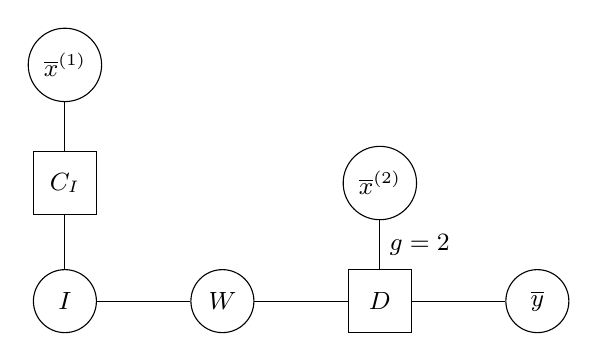
\begin{tikzpicture}[every node/.style={font=\small},
 bus/.style={circle,draw,minimum size=8mm},
 pin/.style={rectangle,draw,minimum size=8mm}]
\node[bus] (I) at (0,0) {$I$};
\node[bus] (W) at (2,0) {$W$};
\node[pin] (D) at (4,0) {$D$};
\node[pin] (C) at (0,1.5) {$C_I$};
\node[bus] (x1) at (0,3) {$\comp{x}^{(1)}$};
\node[bus] (x2) at (4,1.5) {$\comp{x}^{(2)}$};
\node[bus] (y) at (6,0) {$\comp{y}$};
\draw (x1)--(C)--(I)--(W)--(D)--(y);
\draw (D)--node[right] {$g=2$}(x2);
\end{tikzpicture}
\caption{Inversion gadget. Squares have voltage $1$; the three upper or
rightmost value copies belong to variable paths, whose lines are omitted.
Every unmarked line has conductance $1$. Superscripts distinguish buses,
not numerical values.}
\label{fig:inversion}
\end{figure}

The equation at $C_I$ gives
\[
 (1-v_I)+(1-\comp{x})=-1/2,
 \qquad\text{hence }v_I=x.
\]
The injection equation at $I$ is therefore
\begin{equation}
 x\bigl[(x-v_W)+(x-1)\bigr]=-1,
 \qquad v_W=2x-1+1/x.
 \label{eq:inversion-I}
\end{equation}
Division is valid because $x\ge1/2$. At $D$ the equation reads
\begin{equation}
 (1-v_W)+2(1-\comp{x})+(1-\comp{y})=-5/2
 \quad\Longleftrightarrow\quad y=v_W-2x+1.
 \label{eq:inversion-D}
\end{equation}
Together these equations imply $y=1/x$.

Conversely, if $x,y\in[1/2,2]$ and $xy=1$, set $v_I=x$ and
$v_W=h(x):=2x-1+1/x$. Both pinned-bus equations and the injection equation
at $I$ then hold. The voltage bound on $W$ is valid: on $[1/2,2]$,
$h'(x)=2-x^{-2}$ and $h''(x)=2x^{-3}>0$, so its minimum is
$2\sqrt{2}-1$ at $1/\sqrt{2}$ and its maximum is the larger endpoint value,
$h(2)=7/2$. Thus
\begin{equation}
 1<2\sqrt{2}-1\le v_W\le7/2<4.
 \label{eq:W-range}
\end{equation}

\subsection{The complete network and proof of equivalence}

Construct all variable paths and equation gadgets with the allocation rule
above. Path value buses have at most two path lines and one gadget line.
Path pinned buses and $C_I$ have degree two; addition buses and $D$ have
degree three; $I$ and $W$ have degree two. Distinct requested copies and fresh
gadget buses prevent loops and parallel edges. Consequently $G$ is simple and
its maximum degree is three.

Every bus voltage belongs to $[1/2,4]$ and every conductance is at most $2$.
For every voltage vector in the prescribed box, not just the intended
solutions, a free-injection bus satisfies
\begin{equation}
 |\power_i(v)|
 \le v_i\sum_{j:\{i,j\}\in E}g_{ij}|v_i-v_j|
 \le 4\cdot3\cdot2\cdot\frac72=84<85.
 \label{eq:free-bound}
\end{equation}
The free-injection intervals therefore add no restriction inside that box.

\begin{lemma}
\label{lem:reduction-equivalence}
The constructed network is feasible if and only if $S_\Phi\ne\varnothing$.
More precisely, restriction to $(v_{X_x})_{x= x_1,\ldots,x_n}$ is a bijection
from its feasible voltage set onto $S_\Phi$.
\end{lemma}
\begin{proof}
Given a feasible voltage vector, put $x=v_{X_x}$ for each named variable.
Every path pinned bus has exactly its two prescribed neighbors, so its
equation forces successive values to be complementary. Every requested copy
thus has its specified value. The addition equation yields $x+y=z$; equations
\eqref{eq:inversion-I}--\eqref{eq:inversion-D} yield $xy=1$. This recovers a
point of $S_\Phi$.

Conversely, given a point of $S_\Phi$, assign alternating values $x$ and
$5/2-x$ along each variable path, voltage $1$ to every pinned bus, and
$v_I=x$, $v_W=2x-1+1/x$ in each inversion gadget. The preceding algebra
verifies every fixed-injection equation. The voltage bounds follow from the
source interval and~\eqref{eq:W-range}; the remaining injection bounds follow
from~\eqref{eq:free-bound}. An isolated $X_x$ has injection zero and retains
exactly the unconstrained source coordinate $x\in[1/2,2]$.

Finally all bus voltages have been uniquely determined by the recovered
source coordinates: path values alternate, pinned values are fixed, and
\eqref{eq:inversion-I} determines $W$. These two maps are inverse bijections.
\end{proof}

\begin{proof}[Proof of Theorem~\ref{thm:rpf-complete}]
Each equation requests exactly three value copies. With at most two path
extensions per request, the paths contribute at most $12m$ new buses and
$12m$ lines in addition to the $n$ initial buses. An addition adds one
further bus and three lines; an inversion adds four further buses and six
lines. Hence the stated bounds $n+16m$ and $18m$ hold, including unused
variables. All numerical data are exactly those displayed in the theorem.
The number of objects is linear in $n+m$; encoding their indices uses
$O((n+m)\log(n+m+2))$ bits, and the construction is polynomial-time.
Lemma~\ref{lem:reduction-equivalence} and $\ER$-completeness of $\ETRINV$
give hardness. Proposition~\ref{prop:rpf-membership} gives membership.
\end{proof}

\begin{proposition}[Preservation of the solution set]
\label{prop:rational-bijection}
The extension map from source solutions to feasible network voltages in
Lemma~\ref{lem:reduction-equivalence} is a homeomorphism whose forward and
inverse coordinate functions are rational with rational coefficients.
Its inverse is restriction to the buses $X_x$, a coordinate projection.
\end{proposition}
\begin{proof}
The extension map has coordinate functions $x$, $5/2-x$, $1$, and
$2x-1+1/x$. They are rational and continuous because $x\ge1/2$.
The inverse projection is linear and continuous. The statement also holds
for empty solution sets and for unused source coordinates.
\end{proof}

\begin{corollary}
\label{cor:rpf-np}
If $\RPF$ belongs to $\NP$, then $\NP=\ER$. In particular, unless these
classes coincide, not every feasible rational instance has a polynomial-size
certificate verifiable in deterministic polynomial time. The problem belongs
to $\PSPACE$.
\end{corollary}
\begin{proof}
By completeness every problem in $\ER$ reduces to $\RPF$. Membership of
$\RPF$ in $\NP$ would imply $\ER\subseteq\NP$, and
\eqref{eq:complexity-inclusions} gives equality. The certificate formulation
is the definition of $\NP$; the space upper bound follows from the same
inclusions.
\end{proof}

The fixed-data conclusion is stronger than a claim that large numerical
coefficients can be encoded economically: all numerical choices in the
hard instances come from finite sets independent of instance size. Their
combinatorial incidence pattern carries the growing input. The theorem uses
general graphs and signed injection intervals; it makes no assertion here
about a load-only model or a tree restriction.

\section{AC feasibility and the meaning of angle limits}
\label{sec:ac}

The resistive result transfers to an AC model with zero reactive injections.
The transfer requires a consistent real angle at every bus: small principal
angle differences on individual lines need not fit together around a cycle.
We first encode this consistency without transcendental constraints. The
encoding works for every line limit strictly below $\pi$, including limits
larger than $\pi/2$.

\subsection{The AC input model}

Write $\mathrm{i}^2=-1$. On a simple undirected graph, line $\{i,j\}$ has
series admittance $y_{ij}=g_{ij}+\mathrm{i}b_{ij}$, where
$g_{ij}\in\Q_{\ge0}$, $b_{ij}\in\Q$, and $y_{ij}\ne0$. Bus $i$ may have a
shunt admittance $s_i=h_i+\mathrm{i}t_i$, with $h_i\in\Q_{\ge0}$ and
$t_i\in\Q$; absence of a shunt means $h_i=t_i=0$. These are reciprocal
series lines without transformers or phase shifters. A line-charging shunt
at a line endpoint may be included in that bus's shunt sum.
Let $U_i=v_i\exp(\mathrm{i}\theta_i)$, with $v_i>0$ and
$\theta_i\in\R$. With injection positive into the network, the equations are
\begin{equation}
 I_i=s_iU_i+\sum_{j:\{i,j\}\in E}y_{ij}(U_i-U_j),\qquad
 P_i+\mathrm{i}Q_i=U_i\overline{I_i}.
 \label{eq:complex-power}
\end{equation}
The input gives positive rational magnitude bounds $\ell_i\le v_i\le u_i$
and finite rational intervals $[p_i^-,p_i^+]$, $[q_i^-,q_i^+]$ for $P_i,Q_i$.
Singleton intervals are allowed independently for these three quantities.
Every line also has a rational number $c_{ij}\in(-1,1]$, representing
$\gamma_{ij}=\arccos c_{ij}\in[0,\pi)$, and the constraint
\begin{equation}
 |\theta_i-\theta_j|\le\gamma_{ij}.
 \label{eq:real-angle-limit}
\end{equation}
The problem $\ACPF$ asks for $v\in\R_{>0}^N$ and $\theta\in\R^N$ satisfying
these equations and bounds. The rational input contains $c_{ij}$, not an
approximation to $\gamma_{ij}$. Angles may be shifted by a common constant
on each connected component; an optional reference angle zero per component
only fixes this freedom.

For later use, write $U_i=e_i+\mathrm{i}f_i$ and introduce a positive magnitude
variable $r_i$. Define
\begin{equation}
 H_{ij}=e_ie_j+f_if_j,\qquad D_{ij}=f_ie_j-e_if_j.
 \label{eq:dot-cross}
\end{equation}
Thus $D_{ij}=\operatorname{Im}(U_i\overline{U_j})=-D_{ji}$.
Expanding~\eqref{eq:complex-power} gives the polynomial expressions
\begin{align}
 P_i&=h_ir_i^2+\sum_j\bigl[g_{ij}(r_i^2-H_{ij})-b_{ij}D_{ij}\bigr],
 \label{eq:rect-P}\\
 Q_i&=-t_ir_i^2+\sum_j\bigl[-b_{ij}(r_i^2-H_{ij})-g_{ij}D_{ij}\bigr],
 \label{eq:rect-Q}\\
 r_i^2&=e_i^2+f_i^2,\qquad \ell_i\le r_i\le u_i.
 \label{eq:rect-magnitude}
\end{align}
Here and below, line sums run over neighbors of $i$. All these constraints
have rational coefficients and degree at most two.

\subsection{A polynomial encoding of real angle lifts}

For two nonzero phasors with non-antipodal directions, let
$\delta_{ij}\in(-\pi,\pi)$ be the principal argument of
$U_i\overline{U_j}$. The principal-angle limit
$|\delta_{ij}|\le\gamma_{ij}$ is exactly
\begin{equation}
 H_{ij}\ge c_{ij}r_ir_j.
 \label{eq:cosine-test}
\end{equation}
Indeed, $H_{ij}/(r_ir_j)=\cos\delta_{ij}$, and cosine decreases on $[0,\pi]$.
Since $c_{ij}>-1$, antipodal directions are excluded. The positive variables
$r_i$ make squaring unnecessary, so the same test covers negative cosines.
Condition~\eqref{eq:cosine-test} alone does not encode~\eqref{eq:real-angle-limit}.

\begin{lemma}[Short-arc crossing count]
\label{lem:crossing}
Let $U_i,U_j\ne0$ have non-antipodal directions, and traverse the short
oriented arc from $U_j/|U_j|$ to $U_i/|U_i|$. Its signed crossing count of
the positive real ray, counting arrival from the open lower half-plane as
$+1$ and departure into that half-plane as $-1$, is
\begin{equation}
 k_{ij}=\begin{cases}
 1,& f_j<0\le f_i\ \text{and }D_{ij}>0,\\
 -1,& f_i<0\le f_j\ \text{and }D_{ij}<0,\\
 0,&\text{otherwise}.
 \end{cases}
 \label{eq:crossing-rule}
\end{equation}
In particular $k_{ji}=-k_{ij}$. If $\alpha_i,\alpha_j\in[0,2\pi)$ are the
arguments of the endpoints, then
\begin{equation}
 \delta_{ij}=\alpha_i-\alpha_j+2\pi k_{ij}.
 \label{eq:crossing-identity}
\end{equation}
\end{lemma}
\begin{proof}
Put $a=\alpha_i-\alpha_j\in(-2\pi,2\pi)$.
If $a< -\pi$, then $\delta_{ij}=a+2\pi\in(0,\pi)$.
Necessarily $\alpha_j>\pi$ and $\alpha_i<\pi$, so
$f_j<0\le f_i$, and $D_{ij}=r_ir_j\sin\delta_{ij}>0$.
Conversely, $f_j<0\le f_i$ implies $\alpha_j\in(\pi,2\pi)$ and
$\alpha_i\in[0,\pi]$, hence $a<0$. Within $(-2\pi,0)$ the additional
condition $\sin a>0$ holds exactly when $a< -\pi$.
Thus the first case of~\eqref{eq:crossing-rule} is precisely $a< -\pi$.
Reversing $i,j$ proves that its second case is precisely $a>\pi$.
The remaining case has $|a|<\pi$, including $a=0$, and needs no wrap.
The equalities $a=\pm\pi$ are excluded by the non-antipodal hypothesis.
This proves~\eqref{eq:crossing-identity} and reversal symmetry. It also
checks the axis convention: argument zero belongs to the closed upper
half-plane; argument $\pi$ does too, but the determinant sign prevents
counting a crossing of the negative real ray.
\end{proof}

Fix one orientation $j\to i$ for every line. For any directed traversal of
a cycle $C$, write $\varepsilon_{C,ij}=1$ if it traverses that line in its
chosen orientation and $-1$ if it traverses it in reverse. Telescoping the
$\alpha$ terms in~\eqref{eq:crossing-identity} gives
\begin{equation}
 \sum_{\{i,j\}\in C}\varepsilon_{C,ij}\delta_{ij}
 =2\pi\sum_{\{i,j\}\in C}\varepsilon_{C,ij}k_{ij}.
 \label{eq:cycle-winding}
\end{equation}
The integer on the right after division by $2\pi$ is the winding number.

\begin{lemma}[Real-angle lift criterion]
\label{lem:lift}
Suppose~\eqref{eq:cosine-test} holds on every line. There are real angles
$\theta_i$ representing the phasors and satisfying~\eqref{eq:real-angle-limit}
if and only if
\begin{equation}
 \sum_{\{i,j\}\in C}\varepsilon_{C,ij}k_{ij}=0
 \label{eq:zero-winding}
\end{equation}
for each fundamental cycle of a spanning forest of $G$.
\end{lemma}
\begin{proof}
For a real lift within the limits, both $\theta_i-\theta_j$ and
$\delta_{ij}$ belong to $(-\pi,\pi)$ and represent the same argument.
They are therefore equal, and their sum around every cycle is zero.
Equation~\eqref{eq:cycle-winding} proves necessity.
Conversely choose one argument at a root of each tree of the forest and
extend $\theta$ along its edges by $\theta_i-\theta_j=\delta_{ij}$.
These angles represent the given phasors. Each non-tree edge and its
unique forest path form a fundamental cycle. Its zero sum in
\eqref{eq:cycle-winding} forces the same difference equation on that edge.
Every line difference is thus its principal difference and satisfies its limit.
\end{proof}

\begin{theorem}
\label{thm:ac-membership}
The problem $\ACPF$ belongs to $\ER$ for rational cosine limits
$c_{ij}\in(-1,1]$.
\end{theorem}
\begin{proof}
Use variables $e_i,f_i,r_i$ subject to~\eqref{eq:rect-magnitude}, the injection
intervals applied to~\eqref{eq:rect-P}--\eqref{eq:rect-Q}, and
\eqref{eq:cosine-test}. For each oriented line introduce a real $k_{ij}$ and
encode~\eqref{eq:crossing-rule} by a Boolean combination of polynomial
comparisons: either its first condition and $k_{ij}=1$, or its second
condition and $k_{ij}=-1$, or the negations of both conditions and $k_{ij}=0$.
Add~\eqref{eq:zero-winding} for the fundamental cycles.
Lemmas~\ref{lem:crossing}--\ref{lem:lift} prove equivalence to real-angle
feasibility. There are $O(|N|+|E|)$ variables and at most
$|E|-|N|+\kappa$ fundamental cycles, where $\kappa$ is the number of
components. Each cycle has at most $|N|$ edges. Consequently the Boolean
formula and its rational coefficients have polynomial encoding length.
All quantified variables are real; the three-valued crossing variables
require no additional integer quantifier.
\end{proof}

\subsection{Zero reactive injection and the hardness transfer}

For purely resistive lines with $g_{ij}>0$ and no shunts, the polar form of
\eqref{eq:rect-P}--\eqref{eq:rect-Q} is
\begin{align}
 P_i&=\sum_j g_{ij}\bigl(v_i^2-v_iv_j\cos(\theta_i-\theta_j)\bigr),
 \label{eq:resistive-ac-P}\\
 Q_i&=-\sum_j g_{ij}v_iv_j\sin(\theta_i-\theta_j).
 \label{eq:resistive-ac-Q}
\end{align}

\begin{lemma}[Equal angles under a real lift]
\label{lem:equal-angles}
In a purely resistive, shunt-free network, suppose $v_i>0$, $Q_i=0$ at
every bus, and $|\theta_i-\theta_j|<\pi$ on every line. Then angles are
constant on each connected component. The active injections are exactly
$\power_i(v)$ from~\eqref{eq:rpf}. Conversely, every positive resistive
voltage profile extends to an AC profile with these injections and $Q=0$
by taking all angles zero.
\end{lemma}
\begin{proof}
Multiply~\eqref{eq:resistive-ac-Q} by $-\theta_i$ and sum over buses.
Pairing the two contributions of each line yields
\begin{equation}
 0=-\sum_i\theta_i Q_i
 =\sum_{\{i,j\}\in E}g_{ij}v_iv_j
 (\theta_i-\theta_j)\sin(\theta_i-\theta_j).
 \label{eq:angle-energy}
\end{equation}
Each summand is nonnegative, and $t\sin t>0$ for $0<|t|<\pi$.
Since $g_{ij}v_iv_j>0$, every line difference is zero. Substitution in
\eqref{eq:resistive-ac-P} gives~\eqref{eq:rpf}. The converse follows directly
from~\eqref{eq:resistive-ac-P}--\eqref{eq:resistive-ac-Q}.
\end{proof}

The sine balance in~\eqref{eq:resistive-ac-Q} is also the equilibrium equation
of a weighted oscillator network; see \citet{DorflerEtAl2013} for this
connection and cohesive-angle analysis. The elementary identity
\eqref{eq:angle-energy} supplies the exact statement needed here, with real
bus angles and line differences strictly below $\pi$. It does not require
strictly positive cosine or a stability assumption.

\begin{theorem}
\label{thm:ac-complete}
The problem $\ACPF$ is $\ER$-complete. Hardness holds on simple graphs of
maximum degree three, with $b_{ij}=h_i=t_i=0$, $q_i^-=q_i^+=0$ at every bus,
$c_{ij}=0$ on every line, and the fixed finite conductance, magnitude, and
active-injection data of Theorem~\ref{thm:rpf-complete}.
\end{theorem}
\begin{proof}
Take the resistive instance of Theorem~\ref{thm:rpf-complete}, retain its
graph and data, and add the stated AC data. The cosine input zero represents
the real-angle limit $\pi/2$. Lemma~\ref{lem:equal-angles} proves equivalence
in both directions, and Theorem~\ref{thm:ac-membership} proves membership.
\end{proof}

Thus $\ACPF\in\NP$ would imply $\NP=\ER$. This conclusion concerns the
specified AC model with variable magnitudes and resistive lines. It does not
classify the lossless, fixed-magnitude model, whose nonlinear variables are
angles alone.

\begin{corollary}[One-sided reactive intervals]
\label{cor:one-sided-reactive}
Theorem~\ref{thm:ac-complete} remains true if every reactive-injection
interval $[0,0]$ is replaced by the positive-width interval $[0,1]$.
More generally, in a purely resistive, shunt-free network, requiring all
reactive injections to be nonnegative, or all to be nonpositive, forces
each of them to be zero.
\end{corollary}
\begin{proof}
Antisymmetry of the sine terms in~\eqref{eq:resistive-ac-Q} gives
$\sum_i Q_i=0$. Numbers of one common weak sign with zero sum all vanish.
Conversely, zero belongs to $[0,1]$, so the feasible set is unchanged.
\end{proof}

The same replacement applies to the two restricted AC formulations below.
This removes the need to specify singleton reactive intervals, while the
network identity still enforces exact zero reactive injections. It is a
one-sided saturation argument, not a robustness assertion for symmetric
intervals $[-\varepsilon,\varepsilon]$.

\subsection{Principal angles: a counterexample and a positive-window result}
\label{subsec:principal}

Define \emph{principal-angle AC feasibility} by
\eqref{eq:rect-P}--\eqref{eq:cosine-test} and the injection intervals, without
the cycle equations~\eqref{eq:zero-winding}. This is a polynomial feasibility
problem and hence belongs to $\ER$. The distinction from $\ACPF$ is material.

\begin{proposition}[Winding prevents an unrestricted transfer]
\label{prop:winding-counterexample}
On a unit-conductance $n$-cycle, $n\ge3$, the phasors
$U_k=\exp(2\pi\mathrm{i}k/n)$ have unit magnitudes and satisfy
\begin{equation}
 Q_k=0,\qquad P_k=2\bigl(1-\cos(2\pi/n)\bigr)>0.
 \label{eq:cycle-profile}
\end{equation}
Their principal line differences have absolute value $2\pi/n$ and winding
number one. Consequently, for every fixed rational $c\in(-1,1)$ there is a
rational-data instance with line cosine limit $c$ that is principal-angle
AC feasible but whose corresponding resistive instance is infeasible.
\end{proposition}
\begin{proof}
At each bus, the two sine terms in~\eqref{eq:resistive-ac-Q} cancel and the
cosine terms coincide, giving~\eqref{eq:cycle-profile}. The oriented sum
around the cycle is $2\pi$, so Lemma~\ref{lem:lift} excludes a real lift
with these principal differences. Given $c<1$, choose $n\ge3$ large enough
that $2\pi/n\le\arccos c$. Put unit magnitude bounds and zero reactive
injections at all buses, and choose rational numbers $0<a<P_k<b$ as active
injection bounds $[a,b]$. Such numbers exist by density of $\Q$; the powers
in~\eqref{eq:cycle-profile} themselves need not be rational. The phasors
give principal-angle feasibility, whereas every resistive voltage is one
and its injection is zero, outside $[a,b]$.
For an explicit instance with singleton rational injections, take $n=4$,
$c=0$, and $[p_k^-,p_k^+]=[2,2]$.
\end{proof}

This example disproves an equal-angle implication from fixed positive
principal windows; it does not assert a complexity classification for every
such fixed-window class. At the other endpoint, the bound strictly below
$\pi$ in Lemma~\ref{lem:equal-angles} is sharp: a single unit-conductance
line with unit magnitudes and real angles $0,\pi$ has $Q=0$ and active
injection $2$ at both buses.

A positive principal window can nevertheless enforce the needed real lift
when its width is allowed to depend on the graph size.

\begin{lemma}[Small cycle budgets exclude winding]
\label{lem:small-cycle-budget}
Suppose principal angle limits $\gamma_{ij}<\pi$ satisfy
$\sum_{\{i,j\}\in C}\gamma_{ij}<2\pi$ for every fundamental cycle $C$
of some spanning forest. Then every phasor profile satisfying those limits
has a real lift satisfying the same limits.
\end{lemma}
\begin{proof}
The principal difference sum on $C$ is a multiple of $2\pi$ by
\eqref{eq:cycle-winding}. Its absolute value is at most the stated sum of
limits and therefore strictly less than $2\pi$. It must vanish.
Lemma~\ref{lem:lift} applies. In particular, every forest has this property
without any additional restriction on its limits below $\pi$.
\end{proof}

\begin{corollary}[Strictly positive principal windows]
\label{cor:principal-hardness}
Principal-angle AC feasibility is $\ER$-complete even on simple graphs of
maximum degree three with purely resistive lines, no shunts, zero reactive
injections, the fixed numerical data of Theorem~\ref{thm:rpf-complete}, and
the common cosine limit
\begin{equation}
 c_n=1-\frac{1}{n^2},\qquad n=|N|\ge2.
 \label{eq:shrinking-window}
\end{equation}
The angle window is strictly positive. Its cosine has $O(\log n)$ bits;
unlike the other data, these cosines do not belong to a fixed finite set.
\end{corollary}
\begin{proof}
For $t\in[0,\pi]$, concavity of sine on $[0,\pi/2]$ gives
$\sin(t/2)\ge t/\pi$, and therefore
$1-\cos t=2\sin^2(t/2)\ge2t^2/\pi^2$.
Writing $\gamma_n=\arccos c_n$, we obtain
$0<\gamma_n\le\pi/(\sqrt{2}n)$.
Every simple cycle has at most $n$ edges, so the sum of its limits is at
most $\pi/\sqrt{2}<2\pi$. Lemma~\ref{lem:small-cycle-budget} supplies a
real lift, and Lemma~\ref{lem:equal-angles} proves equivalence to the
resistive instance. Take that instance from Theorem~\ref{thm:rpf-complete}.
If needed, add isolated buses with magnitude bounds $[1/2,2]$ and active
injection bounds $[-85,85]$ to ensure $n\ge2$. These buses are feasible
and use the original finite alphabet. Computing~\eqref{eq:shrinking-window} takes
polynomial time. Membership follows from the rectangular formulation.
\end{proof}

\subsection{A rectangular model with bus-angle boxes}
\label{subsec:angle-box}

There is also a hardness transfer using only linear angle restrictions in
rectangular coordinates. Choose a reference bus in each connected component
and require
\begin{equation}
 e_i\ge f_i,\qquad e_i\ge-f_i\quad(i\in N),\qquad
 f_{\mathrm{ref}}=0,\quad e_{\mathrm{ref}}>0.
 \label{eq:angle-box}
\end{equation}
The positive lower magnitude bounds imply $e_i>0$, so these conditions are
exactly the angle box $\theta_i\in[-\pi/4,\pi/4]$ relative to a reference
angle zero. Their real line differences lie in $[-\pi/2,\pi/2]$.

\begin{corollary}
\label{cor:box-hardness}
The rectangular AC feasibility problem with~\eqref{eq:angle-box} is
$\ER$-complete under the same graph, admittance, magnitude, and injection
restrictions as Theorem~\ref{thm:ac-complete}, without separate line-angle
constraints. In this restricted class every feasible profile has $f_i=0$
and $e_i=v_i$ at every bus, and its feasible set is exactly the resistive
voltage set in these coordinates.
\end{corollary}
\begin{proof}
The formulation is polynomial. The box supplies real angles with the
required line differences, so Lemma~\ref{lem:equal-angles} makes them
constant on each component. Its reference angle makes that constant zero.
Conversely every feasible resistive profile with $e_i=v_i$, $f_i=0$
satisfies the box and all AC constraints.
\end{proof}

The three transfers have different input conventions. Real line limits
permit the fixed choice $c_{ij}=0$ and require the winding equations for
membership. Bus-angle boxes give a direct polynomial encoding with fixed
coefficients. Positive principal-only windows give a direct polynomial
encoding with the size-dependent cosine~\eqref{eq:shrinking-window}.
None of these equivalences assumes that small numerical reactive residuals
are exactly zero.

\section{Planarity, unit conductance, and long cycles}
\label{sec:structural}

The arithmetic construction can be made planar without losing its control of
the entire solution set. A subsequent electrical subdivision removes the
conductance $2$ and all short cycles. The restrictions in the next theorem
hold simultaneously.

\begin{theorem}
\label{thm:structural}
For every fixed positive integer $r$, $\RPF$ is $\ER$-complete on connected
simple planar bipartite graphs of maximum degree three and girth at least
$r$, with every conductance equal to $1$. All voltage and injection interval
endpoints belong to finite rational sets depending only on $r$.
Moreover, every bounded $\ETRINV$ solution set is rationally equivalent to
the feasible voltage set of such a network, with inverse given by projection
onto its original variable buses. The network is constructible in polynomial
time from the source instance, for fixed $r$.
\end{theorem}

Here an acyclic graph has infinite girth. In particular, the theorem does not
assert hardness on trees: its hard graphs can have arbitrarily many cycles.
We prove the statement in three steps.

\subsection{Planarizing bounded arithmetic while preserving solutions}

We use the crossover from the proof of
\citet[Theorem 2.1 and Figure 3]{DobbinsEtAl2023}. Its equations are
\begin{equation}
 X+Y=Z,\qquad X+Y'=Z,\qquad X'+Y=Z.
 \label{eq:crossover}
\end{equation}
They force $X'=X$, $Y'=Y$, and $Z=X+Y$, with unique auxiliary values.
Figure~\ref{fig:crossover} gives a planar incidence drawing with the four
wire terminals in crossing order. The bounds matter: the cited planar
feasibility theorem uses a bounded-witness promise. For preservation of
solution sets we instead impose explicit bounds throughout the following
construction.

\begin{figure}[htbp]
\centering
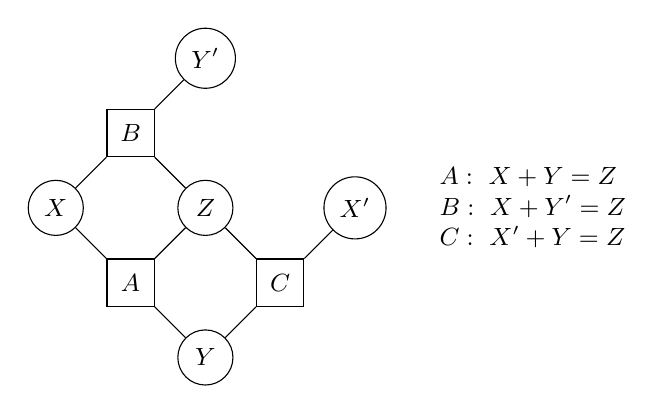
\begin{tikzpicture}[scale=.95,every node/.style={font=\small},
 var/.style={circle,draw,fill=white,minimum size=7mm},
 con/.style={rectangle,draw,fill=white,minimum size=6mm}]
\node[var] (X) at (-2,0) {$X$};
\node[var] (Y) at (0,-2) {$Y$};
\node[var] (Xp) at (2,0) {$X'$};
\node[var] (Yp) at (0,2) {$Y'$};
\node[var] (Z) at (0,0) {$Z$};
\node[con] (A) at (-1,-1) {$A$};
\node[con] (B) at (-1,1) {$B$};
\node[con] (C) at (1,-1) {$C$};
\draw (A)--(X) (A)--(Y) (A)--(Z)
 (B)--(X) (B)--(Yp) (B)--(Z)
 (C)--(Xp) (C)--(Y) (C)--(Z);
\node[anchor=west,align=left] at (3,0)
 {$A:\ X+Y=Z$\\$B:\ X+Y'=Z$\\$C:\ X'+Y=Z$};
\end{tikzpicture}
\caption{An arithmetic crossover. Circles are variables and squares are
equations. The terminal order around the exterior is $X,Y,X',Y'$.
The two transmitted values lie in $[1/2,2]$; only $Z$ needs $[1,4]$.}
\label{fig:crossover}
\end{figure}

\begin{lemma}
\label{lem:bounded-planarization}
From a bounded $\ETRINV$ instance one can construct, in polynomial time,
an addition--inversion system with planar incidence multigraph and variable
intervals in $\{[1/2,2],[1,4]\}$, whose solution set is rationally equivalent
to the original one by a unique extension and coordinate-projection inverse.
All variables in the new system lie in $[1/2,4]$.
\end{lemma}
\begin{proof}
Draw the source incidence multigraph with one edge per variable occurrence,
including repeated occurrences in an equation. A polygonal drawing in general
position with polynomially many crossings can be constructed in polynomial
time: start with distinct rational vertex locations and slightly perturb
straight edges, separating coincident strands and multiple crossing points.
There are only quadratically many pairs of edges. No crossing lies at a vertex.
Regard an edge as a wire transmitting its variable value to that occurrence.
Replace each crossing by~\eqref{eq:crossover} in a disjoint small disk.
Each uninterrupted wire segment carries a variable; at an original variable
vertex all its initial segments carry that original variable. At an original
equation vertex the incident segment values replace the corresponding
occurrences. A segment variable can be placed along its corridor, with its
incidence edges running within that corridor. Figure~\ref{fig:crossover}
shows that all replacements are planar and introduce no further crossings.

Keep every original variable and every transmitted segment value in
$[1/2,2]$. Give each local sum $Z$ the interval $[1,4]$.
The three equations at every crossing force equality of the corresponding
incoming and outgoing values; thus projection recovers precisely the original
bounded system. Conversely, a source assignment has a unique extension:
copy its values along every wire and set each local sum to the sum of its two
wire values. These assignments satisfy the indicated intervals. The maps are
polynomial with rational coefficients in the forward direction and coordinate
projections in the reverse direction, hence continuous. The same reasoning
includes empty solution sets and unused original variables.
\end{proof}

\subsection{A planar electrical realization}

For a system from Lemma~\ref{lem:bounded-planarization}, set $C=9/2$ and
write $\comp{x}=C-x$. This involution preserves $[1/2,4]$.
Use the gadgets of Section~\ref{sec:resistive} with the changes in
Table~\ref{tab:planar-data}. The root bus of each arithmetic variable keeps
its actual source interval; every other path value bus uses $[1/2,4]$.
Thus original and wire variables retain their tighter bounds even though their
electrical copies use the larger interval.

\begin{table}[htbp]
\centering
\begin{tabular}{@{}lll@{}}
\toprule
Bus type & Voltage interval & Fixed injection, if any\\
\midrule
Original or wire root & $[1/2,2]$ & none\\
Crossing-sum root & $[1,4]$ & none\\
Other path value & $[1/2,4]$ & none\\
Copy pin and $C_I$ & $[1,1]$ & $2-C=-5/2$\\
Addition pin & $[1,1]$ & $3-C=-3/2$\\
$I$ & $[1/2,4]$ & $-1$\\
$W$ & $[1,4]$ & none\\
$D$ & $[1,1]$ & $5-3C=-17/2$\\
\bottomrule
\end{tabular}
\caption{Data for the planar construction. ``None'' means the same redundant
interval $[-85,85]$ as before. Gadget lines and conductances are unchanged.}
\label{tab:planar-data}
\end{table}

The copy equation is $a+b=C$, and the addition equation is
$x+y+\comp{z}=C$. At an inversion gadget, $C_I$ gives $v_I=x$,
the equation at $I$ gives $v_W=h(x)=2x-1+1/x$, and the equation at $D$ is
\[
 4-v_W-2(C-x)-(C-y)=5-3C,
 \qquad\text{hence }y=v_W-2x+1=1/x.
\]
If $x,y\in[1/2,4]$ satisfy $xy=1$, then in fact both lie in $[1/2,2]$.
Therefore the previously proved bound~\eqref{eq:W-range} still guarantees
the voltage interval on $W$ in every source solution. This argument is only
needed for solutions; the enlarged construction does not claim that $h(x)$
lies in $[1,4]$ for every $x\in[1/2,4]$.

To preserve planarity, choose the order of requests on each variable path
from its incidence embedding, rather than from the order of equations in an
input list. Take disjoint disks about all incidence vertices and narrow
disjoint corridors about their edges. Around a variable disk, list the
occurrence ports in their cyclic order, breaking that order at any point.
Run its alternating copy path just inside the boundary in this linear order;
insert up to two path extensions to supply each requested parity.
Place each requested value bus at its port. Unrequested intermediate value
buses and pinned buses lie between successive ports, and the path has a break
between its last and first ports. It therefore encloses no region that would
obstruct a corridor. Each requested bus has just one outward gadget line.

An addition disk contains a three-leaf star. An inversion disk contains the
tree of Figure~\ref{fig:inversion}, with three external leaves: two distinct
complemented copies of $x$ and one of $y$. Replace the $x$ incidence corridor
by two adjacent strands. A tree with three specified leaves can be embedded
in a disk with those leaves in either cyclic order (reflect an embedding if
needed); with three leaves these are all cyclic orders. Thus its required
ports can be joined without crossings. If names coincide, keep the
occurrences as adjacent distinct strands within their incidence corridors
and allocate distinct path buses. The same construction handles a normalized
equation $xx=1$; it never identifies its three external buses.

This disk-and-corridor substitution proves planarity, simplicity, and maximum
degree three. Every free injection remains redundant by~\eqref{eq:free-bound}.
All fixed-injection equations have the same reversible algebra as before,
so extension to network voltages is rational, unique, and continuous, with
the arithmetic root voltages as inverse projection. The finite data sets
are explicitly given in Table~\ref{tab:planar-data}, together with
conductances $1,2$ and the free injection interval.

\begin{lemma}
\label{lem:connect}
The networks just constructed can be made connected and planar, preserving
their rational solution-set correspondence, degree bound, and finite data.
\end{lemma}
\begin{proof}
Each nonempty component contains an arithmetic root bus. That root is an
endpoint of its copy path and receives at most one gadget line, so its degree
is at most two; its injection is free. In each component choose one such root,
add a new bus of voltage $1$ and free injection, and join it to that root by
a unit-conductance line. Join the new buses in a path, also with unit
conductance. Every modified degree is at most three. Modified old injections
and all new injections satisfy~\eqref{eq:free-bound} throughout the voltage
box; the lines between new buses have zero voltage drop. Thus no constraint
on old voltages changes, and the new voltages are uniquely fixed.

For planarity, the chosen root is incident with some face of its component;
choose that face as the exterior face before arranging the components in
disjoint disks along the new path. Each root-to-new-bus line can leave its
component through this face, and the path runs outside the disks. This gives
a planar drawing. If the arithmetic system has no variables, its solution
set is the single point of $\R^0$; use one isolated voltage-$1$ bus with
injection zero. This also meets all claims, allowing the singleton interval
$[0,0]$ in the fixed injection alphabet.
\end{proof}

\subsection{Electrical subdivision}

\begin{lemma}
\label{lem:subdivision}
Fix a positive integer $L$. In any network above, replace each conductance-$1$
line by a path of $4L$ unit-conductance lines, and each conductance-$2$ line
by a path of $2L$ unit-conductance lines. Give each new internal bus voltage
interval $[1/2,4]$ and injection zero, and divide every old injection interval
by $4L$. The new feasible voltage set is rationally equivalent to the old
one by affine extension and coordinate-projection inverse. The new graph is
simple, bipartite, and has girth at least $6L$; connectedness, planarity, and
the maximum-degree-three bound are preserved.
\end{lemma}
\begin{proof}
Consider a replacement path of length $s$ with endpoint voltages $a,b$.
Its positive internal voltages and zero injections give
$2v_j-v_{j-1}-v_{j+1}=0$. Hence uniquely
\[
 v_j=(1-j/s)a+(j/s)b\qquad(0\le j\le s).
\]
These convex combinations lie in $[1/2,4]$. The endpoint current is
$(a-b)/s$, equal to the old line current divided by $4L$. Summing at each
old bus proves that its new injection is its old injection divided by $4L$.
This proves both directions and the affine correspondence.

Subdivision preserves planarity and connectedness and does not increase old
degrees. All internal degrees are two. Since every path length is even,
color all old vertices alike and alternate colors along each path to obtain
a bipartition. Every simple cycle in the new graph traverses full replacement
paths and projects to a simple cycle in the old simple graph, which has at
least three edges. Each path has at least $2L$ edges, proving the girth bound.
For fixed $L$, the construction has linear size in the old graph and retains
a finite data alphabet, obtained by scaling the old injection endpoints and
adjoining zero.
\end{proof}

\begin{proof}[Proof of Theorem~\ref{thm:structural}]
Apply bounded planarization, the planar electrical realization, and
Lemma~\ref{lem:connect}. Then apply Lemma~\ref{lem:subdivision} with
$L=\max\{1,\lceil r/6\rceil\}$. Every step preserves the entire solution
set by a rational homeomorphism whose inverse reads earlier coordinates.
All steps have polynomial size for fixed $r$. Hardness follows from
$\ETRINV$, and membership remains Proposition~\ref{prop:rpf-membership}.
\end{proof}

\begin{corollary}
\label{cor:structural-ac}
The graph and conductance restrictions of Theorem~\ref{thm:structural}
also hold simultaneously for the AC hardness results with fixed real-angle
limits and for the bus-angle-box model. All numerical data can again be
chosen from fixed finite sets. They also hold for the principal-only model
of Corollary~\ref{cor:principal-hardness}, whose positive cosine limit has
polynomial bit length and depends on the final number of buses.
\end{corollary}
\begin{proof}
Apply the corresponding AC transfer to the final subdivided network.
For the principal-only transfer, every source with a named variable already
produces at least two buses after connection and subdivision, so no isolated
padding is needed. For the zero-variable source, instead use two voltage-$1$
buses with zero active and reactive injections, joined by one unit-conductance
line, and set $c_2=3/4$. This graph is connected, simple, planar, and bipartite,
with degree one and infinite girth; its feasible magnitude set is a singleton.
Apart from this exception, the transfers change no graph or conductance and
preserve the feasible voltage magnitudes. Zero reactive injections may also
be replaced by the one-sided intervals of
Corollary~\ref{cor:one-sided-reactive}.
\end{proof}

\section{Feasible-set universality and exact algebraic voltages}
\label{sec:algebraic}

The reduction preserves more than a yes-or-no answer. Its rational
solution-set correspondence transfers both topology and fields of definition.
We call two real sets \emph{rationally equivalent} if there is a
homeomorphism between them whose coordinate functions, and those of its
inverse, are rational functions with rational coefficients, with denominators
nonzero on their respective domains.
A set is \emph{basic closed over $\Q$} if it is described by a finite
conjunction of polynomial equalities and weak inequalities with rational
coefficients. General semialgebraic descriptions may also use disjunctions
and strict inequalities. This distinction matters for rational equivalence.

\begin{lemma}[Bounded arithmetic for basic closed sets]
\label{lem:basic-arithmetic}
Every compact basic closed set $S\subseteq\R^d$ over $\Q$ is rationally
equivalent to the solution set of a bounded $\ETRINV$ instance.
The equivalence can retain, for every original coordinate $t_i$, a designated
replacement coordinate $x_{j(i)}=1+\varepsilon t_i$, where
$\varepsilon>0$ is rational. All added coordinates are uniquely determined
rational functions of the original coordinates.
\end{lemma}

Appendix~\ref{app:arithmetic} proves the lemma using the conjunction-only
arithmetic constructions underlying Lemmas C--G of
\citet{AbrahamsenMiltzow2019}. It gives the gate identities, checks their
ranges, and avoids Boolean preprocessing. We assert existence here, without
a size bound for an arbitrary description of $S$.

\begin{theorem}
\label{thm:universality}
A compact semialgebraic set defined over $\Q$ is rationally equivalent
to the feasible voltage set of a rational $\RPF$ instance if and only if
it is basic closed over $\Q$.
For every prescribed fixed girth bound, the instance can satisfy all the
structural and finite-data restrictions of Theorem~\ref{thm:structural}.
\end{theorem}
\begin{proof}
For sufficiency, compose Lemma~\ref{lem:basic-arithmetic} with
Proposition~\ref{prop:rational-bijection}, or with the stronger construction
of Theorem~\ref{thm:structural}. Composition preserves rationality and
continuity in both directions. Necessity follows from
Proposition~\ref{prop:basic-invariance} below, because every rational RPF
voltage set is basic closed over $\Q$. Empty sets are included.
\end{proof}

\begin{proposition}[Basic closedness is preserved]
\label{prop:basic-invariance}
If a compact set $S$ is rationally equivalent over $\Q$ to a basic closed
set $T$ over $\Q$, then $S$ is basic closed over $\Q$.
\end{proposition}
\begin{proof}
The empty case is immediate. Otherwise write the equivalence and its
inverse as $F:S\to T$ and $G:T\to S$. Collect the polynomial denominators
of the coordinates of $F$. For each denominator of $G$, substitute $F$
and clear the forward denominators, without cancellation, to obtain a
polynomial numerator. Add these numerators to the collection. Every
collected polynomial is nonzero on $S$. Compactness supplies a rational
$\eta>0$ smaller than all their absolute values on $S$.

Let $S'$ consist of all ambient points $t$ satisfying three conditions:
every collected polynomial has square at least $\eta^2$;
$F(t)\in T$; and $G(F(t))=t$. The first condition makes all expressions
in the other two well defined. Clearing their denominators by positive
even powers turns them into polynomial equalities and weak inequalities
over $\Q$. Hence $S'$ is basic closed. The inverse identities give
$S\subseteq S'$. Conversely, if $t\in S'$, then $F(t)\in T$ and
$t=G(F(t))\in S$. Thus $S'=S$.
\end{proof}

The restriction in Theorem~\ref{thm:universality} cannot be dropped.
Consider the compact three-quadrant set
\begin{equation}
\label{eq:three-quadrants}
 S=[-1,1]^2\cap\bigl(\{(x,y):x\ge0\}\cup\{(x,y):y\ge0\}\bigr).
\end{equation}
It is not even locally basic closed at the origin. To see this, suppose
finitely many polynomial weak inequalities describe it near the origin;
equalities can be replaced by pairs of inequalities. Every nonzero
defining polynomial $p$ with $p(0)=0$ has a lowest nonzero homogeneous
part $H$ that is nonnegative in the three included open quadrants.
Its degree cannot be odd: the second and fourth quadrants are negatives
of each other, which would force $H$ to vanish on an open set.
Its degree is therefore even, so $H$ is nonnegative in the
remaining quadrant as well. Choose a direction in the excluded lower-left
quadrant avoiding the zero sets of these finitely many nonzero homogeneous
polynomials. All their values there are strictly positive. Along a
sufficiently short segment of that ray, every $p$ is positive; polynomials
with positive constant term also remain positive, and zero polynomials
impose no condition. This contradicts exclusion of that segment.

\begin{theorem}[Topological universality]
\label{thm:topological-universality}
Every compact semialgebraic set is semialgebraically homeomorphic to the
voltage feasible set of a rational RPF instance satisfying all restrictions
of Theorem~\ref{thm:structural}, for any prescribed fixed girth bound.
The homeomorphism need not be rational.
\end{theorem}
\begin{proof}
The empty case follows from Theorem~\ref{thm:universality}. A nonempty
compact semialgebraic set has a semialgebraic triangulation by a finite
simplicial complex $K$; see \citet[Theorem 1.1 and Section 1.2]{OhmotoShiota2017}.
Let its vertices be $1,\ldots,N$. The standard simplex realization of $K$ is
\begin{equation}
\label{eq:simplex-nonfaces}
 T_K=\left\{z\in\R^N:
 z_i\ge0,\quad \sum_i z_i=1,\quad
 \prod_{i\in F}z_i=0\ \text{for every nonface }F\subseteq\{1,\ldots,N\}
 \right\}.
\end{equation}
The support of $z$ is a face exactly when all the nonface equations hold.
Thus $T_K$ is the union of the standard simplices indexed by $K$.
The barycentric map from these standard simplices to any geometric
realization of $K$ is a piecewise linear homeomorphism: it is affine and
bijective on each simplex, and these maps agree on common faces.
Consequently $T_K$ is semialgebraically homeomorphic to the original set.
It is compact and basic closed over $\Q$, so
Theorem~\ref{thm:universality} applies. No bound on the size of the
triangulation or the list of nonfaces is asserted.
\end{proof}

The structured voltage sets therefore need not be connected, contractible,
or zero-dimensional. The equal-angle AC transfers preserve these magnitude
sets. Fixing a reference angle in each connected component gives the same
conclusions for rectangular voltages in the bus-angle-box model. Rational
equivalence retains algebraic information that a semialgebraic
homeomorphism can change; this is why the two universality statements
have different scopes.

\begin{theorem}
\label{thm:algebraic-degree}
Let $\alpha$ be a real algebraic number. There is a rational $\RPF$
instance with a unique feasible voltage vector $v$ such that every $v_i$
belongs to $\Q(\alpha)$ and $\Q(v_j)=\Q(\alpha)$ for some designated bus
$j$. Consequently, a uniquely feasible rational network can have a designated
bus voltage of any prescribed algebraic degree over $\Q$.
All structural restrictions of Theorem~\ref{thm:structural} can be imposed.
The same statement holds for unique AC magnitudes, and for unique rectangular
voltages in the reference-fixed bus-angle-box model.
\end{theorem}
\begin{proof}
First suppose $\alpha\notin\Q$. Choose a nonzero polynomial in $\Q[t]$
having $\alpha$ as a root and rational endpoints $a<b$ whose interval
contains $\alpha$ and no other root. Its root condition together with
$a\le t\le b$ defines the singleton $\{\alpha\}$.
Lemma~\ref{lem:basic-arithmetic} gives a bounded $\ETRINV$
solution set rationally equivalent to this singleton, so it too is a
singleton, say $\{x\}$. Rationality of the forward map gives
$x_i\in\Q(\alpha)$ for every coordinate.

The designated-coordinate conclusion of the lemma recovers an original
coordinate by a rational affine rescaling of one replacement coordinate. Thus
$\alpha=A x_j+B$ for some $A,B\in\Q$. Since $\alpha$ is irrational,
$A\ne0$, and hence $\Q(x_j)=\Q(\alpha)$.
The network construction has a unique extension of $x$, with rational
coordinate functions, and it retains $x_j$ as the voltage at its original
variable root. The planarization, connectors, and subdivisions retain that
root coordinate and add only uniquely determined rational functions of the
old coordinates. This proves the claims for irrational $\alpha$.

For rational $\alpha$, a single voltage-$1$, zero-injection bus is sufficient:
its unique voltage generates $\Q=\Q(\alpha)$ and its graph meets every
stated restriction. To obtain degree $d\ge2$, take the positive real root
of $t^d-2$; this polynomial is irreducible by Eisenstein's criterion at $2$.
Degree one is the preceding rational example. Finally, the exact AC transfers
preserve precisely the RPF magnitude set, and reference-fixed angle boxes
force every phase to zero.
\end{proof}

The designated-coordinate assertion uses the affine recovery property,
not merely preservation of the field generated by all coordinates. The
theorem is an existence statement and asserts no additional size bound on
the affine recovery coefficients. It also does not by itself exclude
polynomially verifiable symbolic certificates: the relevant obstruction to
such certificates is the complexity consequence in
Corollary~\ref{cor:rpf-np}.

\section{Residuals, approximate certificates, and reactive stability}
\label{sec:numerical}

Exact feasibility and small residuals answer different questions. We make
their relationship explicit, first for the arithmetic reduction and then
for general bounded resistive networks. Throughout this section the voltage
bounds remain exact, including singleton bounds at pinned buses. Only
injection constraints are relaxed.

For a nonempty rational voltage box $B=\prod_i[\ell_i,u_i]$, define
\begin{equation}
 \rho_G(v)=\max_i\operatorname{dist}
       (\power_i(v),[p_i^-,p_i^+]),\qquad
 \gamma_G=\min_{v\in B}\rho_G(v).
 \label{eq:network-residual}
\end{equation}
Continuity and compactness imply that the minimum is attained and that
$\gamma_G=0$ exactly when the network is feasible. For a normalized source
instance $\Phi$, define
\begin{equation}
 R_\Phi(x)=\max\bigl\{|x+y-z|:\ x+y=z\text{ in }\Phi;
             \ |xy-1|:\ xy=1\text{ in }\Phi\bigr\},
 \qquad \gamma_\Phi=\min_{x\in[1/2,2]^n}R_\Phi(x).
 \label{eq:source-residual}
\end{equation}
A maximum over no constraints is zero, including for an empty network.

\subsection{A quantitative correspondence for the actual gadgets}

\begin{theorem}
\label{thm:residual-transfer}
For the ordinary construction of Section~\ref{sec:resistive}, with $m$
normalized equations,
\begin{equation}
 \frac{\gamma_\Phi}{10(6m+1)}\ \le\ \gamma_G
       \ \le\ 2\gamma_\Phi.
 \label{eq:residual-transfer}
\end{equation}
\end{theorem}
\begin{proof}
Given any source-box point $x$, extend it using exact complementary copies,
$v_I=x$, and $v_W=h(x)=2x-1+1/x$, whether or not it solves $\Phi$.
The voltage bounds hold by~\eqref{eq:W-range}. The free-injection bounds
are redundant throughout the box. All copy, $C_I$, and $I$ equations hold
exactly. An addition bus has residual $|x+y-z|$, and an inversion bus $D$
has residual $|y-1/x|\le2|xy-1|$. Taking a minimizing source point gives
the upper bound.

Conversely, let a network-box point have residual $\varepsilon$ and read
each source variable at its root. A copy pin has voltage exactly $1$, so its
injection residual bounds the error in its neighboring complement sum by
$\varepsilon$. There are at most $6m$ path extensions in the whole network.
Induction along a path therefore shows that each requested copy differs from
its intended root value or complement by at most
$\delta=6m\varepsilon$. The addition equation now gives source residual
at most $\varepsilon+3\delta$.

In an inversion gadget, write $x,y$ for the two root values. The residual
at $C_I$ gives $|v_I-x|\le\varepsilon+\delta$. Dividing the residual at
$I$ by $v_I\ge1/2$ gives
\[
 |v_W-h(v_I)|\le2\varepsilon.
\]
On $[1/2,2]$, $|h'|\le2$, so
$|v_W-h(x)|\le2\varepsilon+2(\varepsilon+\delta)$.
The residual at $D$, including its $x$ copy of weight two and its $y$
copy of weight one, gives
\[
 |y-(v_W-2x+1)|\le\varepsilon+3\delta.
\]
Combining these inequalities and $x\le2$ yields
\[
 |xy-1|\le2\bigl(\varepsilon+3\delta+2\varepsilon
                        +2(\varepsilon+\delta)\bigr)
           =10\varepsilon+10\delta.
\]
This also bounds every addition residual. Apply the resulting inequality
$\gamma_\Phi\le10(6m+1)\rho_G(v)$ to a minimizing network-box point.
If $m=0$, both residual minima are zero and the conclusion still holds.
\end{proof}

The theorem bounds the loss in transferring a residual; it does not supply
a lower bound on $\gamma_\Phi$ for arbitrary infeasible formulas. In fact,
even the fixed-data networks of Section~\ref{sec:resistive} can have
extremely small positive residual minima.

\subsection{Infeasible fixed-data networks with doubly exponential accuracy}

\begin{theorem}
\label{thm:tiny-residual}
For every integer $k\ge0$ there is an infeasible connected network $G_k$
with the fixed numerical data and degree bound of
Theorem~\ref{thm:rpf-complete}, at most $68k+67$ buses and $72k+72$
lines, and a rational voltage vector in its exact voltage box for which
every injection constraint except one holds exactly and
\begin{equation}
 0<\gamma_{G_k}\le\rho_{G_k}(v)<2^{-2^k}.
 \label{eq:tiny-residual}
\end{equation}
The strict lower bound concerns the minimum; the exhibited residual is only
an upper bound on that minimum.
\end{theorem}
\begin{proof}
Use the variables $t,h,x_0,\ldots,x_k$ and
$a_j,b_j,c_j$ for $0\le j<k$, all in $[1/2,2]$. Impose
\begin{equation}
\begin{gathered}
 tt=1,\qquad h+h=t,\qquad t+h=x_0,\\
 a_j+h=x_j,\quad x_jb_j=1,\quad a_j+b_j=c_j,\quad x_{j+1}+h=c_j
                 \quad(0\le j<k),\\
 x_kt=1.
\end{gathered}
 \label{eq:tiny-system}
\end{equation}
The first three equations force $t=1$, $h=1/2$, $x_0=3/2$.
Each group of four then forces
\[
 x_{j+1}=x_j+1/x_j-1.
\]
Writing $x_j=1+\delta_j$ gives
$\delta_0=1/2$ and
$\delta_{j+1}=\delta_j^2/(1+\delta_j)>0$.
The last equation requires $x_k=1$, a contradiction.

Nevertheless, assign precisely these recurrence values and set
$a_j=x_j-1/2$, $b_j=1/x_j$, and $c_j=x_j+1/x_j-1/2$.
Then
\[
 1<x_j\le3/2,\quad 1/2<a_j\le1,\quad
 2/3\le b_j<1,\quad 3/2<c_j\le5/3,
\]
so every voltage-source bound holds. All source equations except the last
hold exactly. More explicitly, $\delta_j=1/d_j$, where
$d_0=2$ and $d_{j+1}=d_j(d_j+1)$. Induction gives
$d_k\ge2^{2^k}$.

Apply the ordinary electrical construction and its canonical extension to
this nonsolution. The proof of Theorem~\ref{thm:residual-transfer} shows
that only the final inversion bus $D$ violates its injection constraint,
by exactly
\[
 1-1/x_k=\frac{1}{d_k+1}<2^{-2^k}.
\]
All voltage intervals hold exactly. The source system is infeasible, hence
so is the network, and compactness of its voltage box makes its residual
minimum strictly positive. There are $4k+3$ variables and $4k+4$ equations;
the size bounds follow from Theorem~\ref{thm:rpf-complete}.
The source incidence graph is connected, and each variable path and equation
gadget is connected with all incidence attachments present. Thus the network
is connected as well.
\end{proof}

Its standard graph encoding has length $O((k+1)\log(k+2))$. Therefore no
bound of the form $2^{-\operatorname{poly}(s)}$, with $s$ the input length,
can be a universal lower bound on positive residual minima in this fixed-data
class. Ruling out these infeasible instances solely by a universal residual
threshold can require exponentially many accuracy bits in the number of
buses. This is not a lower bound on exact decision algorithms: the displayed
family has the short algebraic infeasibility proof just given.

There is also a general lower bound at the doubly exponential scale. We
record it to identify the scale of the preceding construction, using a
general theorem about polynomial minima.

\begin{proposition}
\label{prop:residual-separation}
For a rational network with $n\ge1$ buses, put $q=n+1$.
There is an explicitly constructible integer coefficient bound $H$ with
polynomial bit length in the input such that, with
$M=4n+2$, $\widetilde H=\max\{H,2q+2M\}$, and
$\tau=\lceil\log_2\widetilde H\rceil$, infeasibility implies
\begin{equation}
 \gamma_G\ge 2^{-q4^q(\tau+q+4)}.
 \label{eq:separation}
\end{equation}
For fixed-data bounded-degree networks this yields
$\log_2(1/\gamma_G)\le2^{O(n)}$ whenever $0<\gamma_G<1$.
Together with Theorem~\ref{thm:tiny-residual}, the worst-case scale of
this logarithm in that class is $2^{\Theta(n)}$.
\end{proposition}
\begin{proof}
Let $U=\max_i u_i$, $D=\max_i\sum_j g_{ij}$, and
$A=\max_i\max\{|p_i^-|,|p_i^+|\}$.
On the positive voltage box, $|\power_i(v)|\le U^2D$, so
$B_0=1+U^2D+A$ bounds $\rho_G$ from above. Consider the compact set
\[
 T=\{(v,t):v\in B,\ 0\le t\le B_0,\
             t\ge p_i^- -\power_i(v),\
             t\ge\power_i(v)-p_i^+\ (i\in N)\}.
\]
It is connected: each point joins vertically to $(v,B_0)$, and the whole
top face $B\times\{B_0\}$ lies in $T$ and is convex. The minimum of
the polynomial $t$ on $T$ is $\gamma_G$.
There are $M=4n+2$ weak polynomial inequalities, of degree at most two.
Clear denominators in each by a positive integer, and let $H\ge1$ bound
the absolute values of the resulting integer coefficients, also including
the objective $t$. Rational arithmetic gives $\log H$ polynomial in the
input length.

The polynomial-minimum bound of
\citet[Theorem 1.1]{JeronimoEtAl2013}, applied in dimension $q\ge2$
with even degree bound $d=2$, gives for a nonzero minimum
\[
 \gamma_G\ge
  \bigl(2^{4-q/2}\widetilde H\,2^q\bigr)^{-q4^q}.
\]
The logarithm of the base is at most $\tau+q+4$, proving
\eqref{eq:separation}. With a fixed rational data alphabet and bounded
degree, $B_0$ and the cleared coefficient bound can be chosen constant.
Then $\tau=O(\log(n+2))$, and the upper estimate on
$\log_2(1/\gamma_G)$ follows. For the lower estimate, the family above
has linearly many buses in $k$ (in particular its distinct variable roots
number $4k+3$), and its logarithmic residual exceeds $2^k$.
\end{proof}

\subsection{Short rational certificates for a gap promise}

\begin{proposition}
\label{prop:approx-certificates}
Let $\varepsilon>0$ be rational. Every exactly feasible rational $\RPF$
instance has a rational voltage vector in its exact box with
$\rho_G(v)\le\varepsilon/2$, of bit length polynomial in the network input
and the encoding length of $\varepsilon$. Consequently, the promise problem
whose yes cases have $\gamma_G=0$ and whose no cases have
$\gamma_G>\varepsilon$ has polynomial-size certificates verifiable in
deterministic polynomial time. No answer is prescribed when
$0<\gamma_G\le\varepsilon$.
\end{proposition}
\begin{proof}
An empty network is an immediate yes instance and needs no voltage
coordinates. Otherwise put $U=\max_i u_i$ and
$D=\max_i\sum_jg_{ij}$.
For $v,w$ in the voltage box, differentiating~\eqref{eq:rpf} gives
\[
 \left|\frac{\partial\power_i}{\partial v_i}\right|
       \le3UD,
 \qquad
 \sum_{j\ne i}\left|\frac{\partial\power_i}{\partial v_j}\right|
       \le UD.
\]
The segment between $v$ and $w$ remains in the box, so
\begin{equation}
 |\power_i(v)-\power_i(w)|\le4UD\|v-w\|_\infty.
 \label{eq:lipschitz}
\end{equation}
The distance to an interval is $1$-Lipschitz, and the same bound holds for
the change of $\rho_G$.
Choose a dyadic mesh $\eta=2^{-b}$ with
$\eta\le\varepsilon/(2\max\{1,4UD\})$ and $b\ge0$.
Round each coordinate of an exactly feasible point down to this mesh and
then clamp it to its own rational interval. The resulting point stays in
the box, moves by at most $\eta$, and has residual at most
$\varepsilon/2$. Singleton bounds are preserved by clamping. The exponent
$b$ and all resulting rational-coordinate lengths are polynomial in the
input encoding and in that of $\varepsilon$.

A verifier checks the exact rational voltage bounds and evaluates all
injections with rational arithmetic, accepting when the residual is at most
$\varepsilon/2$. The stated bit bound gives completeness on promised yes
instances. No certificate can be accepted when $\gamma_G>\varepsilon$,
giving soundness on promised no instances.
\end{proof}

This is a certificate-existence result, not an algorithm for finding such
a point. It does not put exact $\RPF$ in $\NP$, nor does it decide all
instances of an unpromised approximate feasibility problem at a sharp
tolerance. In particular, it does not resolve the approximate-membership
question of \citet[Section 1.3]{BienstockVermaPreprint2019}:
their question relaxes sine equations in a lossless, fixed-magnitude model
and does not impose the promise used here.

\subsection{Stability of the equal-angle transfer}

The exact reactive argument also has a quantitative version. It applies to
real bus angles with short edge differences; a principal-angle winding
solution does not satisfy that hypothesis.

\begin{proposition}
\label{prop:reactive-stability}
Consider a connected purely resistive AC network with no shunts and $n\ge2$
buses. Let $0<\ell\le v_i\le U$, and suppose the real angle differences on
all lines lie in $[-\pi/2,\pi/2]$. Center the angles so that
$\sum_i\theta_i=0$, let $q$ be their reactive-injection vector, and let
$\lambda_2>0$ be the smallest positive eigenvalue of the conductance
Laplacian $L_g$. Then
\begin{align}
 \|\theta\|_2&\le
       \frac{\pi\|q\|_2}{2\ell^2\lambda_2},
       \label{eq:angle-stability}\\
 0\le P_i(v,\theta)-\power_i(v)&\le
       \frac{\pi^2U^2\|q\|_2^2}{8\ell^4\lambda_2}
       \qquad(i\in N).
       \label{eq:active-stability}
\end{align}
One may replace the constants $\pi/2$ and $\pi^2/8$ by the rational
constants $2$ and $2$, respectively. Moreover,
\begin{equation}
 \lambda_2\ge\frac{2g_{\min}}{(n-1)^2},
 \qquad g_{\min}=\min_{\{i,j\}\in E}g_{ij}.
 \label{eq:spectral-lower}
\end{equation}
Thus entirely rational bounds can be computed directly from the graph data.
For disconnected networks these statements apply componentwise. An isolated
bus has $q_i=0$ and zero active discrepancy.
\end{proposition}
\begin{proof}
Put $s=\theta^TL_g\theta=\sum_{\{i,j\}}g_{ij}(\theta_i-\theta_j)^2$.
The energy identity~\eqref{eq:angle-energy} and
$t\sin t\ge(2/\pi)t^2$ for $|t|\le\pi/2$ give
\[
 (2/\pi)\ell^2s\le-\theta^Tq
       \le\|\theta\|_2\|q\|_2
       \le\sqrt{s/\lambda_2}\,\|q\|_2.
\]
If $s=0$, the centered angles vanish and both conclusions are immediate.
Otherwise divide by $\sqrt s$ to obtain
$s\le\pi^2\|q\|_2^2/(4\ell^4\lambda_2)$, which also gives
\eqref{eq:angle-stability}. From~\eqref{eq:resistive-ac-P} and
$0\le1-\cos t\le t^2/2$,
\[
 0\le P_i(v,\theta)-\power_i(v)
   =\sum_jg_{ij}v_iv_j(1-\cos(\theta_i-\theta_j))
   \le (U^2/2)s.
\]
This proves~\eqref{eq:active-stability}. Using the weaker inequality
$t\sin t\ge t^2/2$ gives the stated rational constants.

Finally, along a simple path of at most $n-1$ edges, Cauchy--Schwarz gives
$(\theta_i-\theta_j)^2\le(n-1)s/g_{\min}$.
For centered angles,
\[
 \|\theta\|_2^2=\frac1n\sum_{i<j}(\theta_i-\theta_j)^2
       \le\frac{(n-1)^2}{2g_{\min}}s.
\]
Minimizing the Rayleigh quotient over nonzero centered vectors proves
\eqref{eq:spectral-lower}. Components can be centered independently because
the electrical quantities depend only on edge differences.
\end{proof}

\begin{corollary}
\label{cor:ac-residual-transfer}
Consider an AC instance obtained from the ordinary $m$-equation resistive
construction, with $n\ge1$ buses, real line differences in
$[-\pi/2,\pi/2]$, and exact voltage bounds. If a state has active-injection
interval violation at most $\varepsilon$ and $\|q\|_\infty\le\eta$, its
root voltage assignment has source residual at most
\begin{equation}
 10(6m+1)\bigl(\varepsilon+256n(n-1)^2\eta^2\bigr).
 \label{eq:ac-residual-transfer}
\end{equation}
\end{corollary}
\begin{proof}
Here $\ell=1/2$, $U=4$, and $g_{\min}\ge1$ in every nonsingleton
component. The rational bounds of Proposition~\ref{prop:reactive-stability},
and $\|q\|_2^2\le n\eta^2$, bound the active discrepancy by
$256n(n-1)^2\eta^2$, also for smaller components. Subtracting this
discrepancy from the actual AC injections bounds $\rho_G(v)$ by the
parenthesis in~\eqref{eq:ac-residual-transfer}. The pointwise reverse
estimate proved in Theorem~\ref{thm:residual-transfer} gives the result.
Singleton components have zero discrepancy, including the case $n=1$.
\end{proof}

These estimates quantify the equal-angle argument by elementary energy and
Poincar\'e inequalities. They control the error induced by a small reactive
residual, but establish neither hardness with symmetric positive reactive
tolerances nor the absence of the winding solutions in
Proposition~\ref{prop:winding-counterexample}.

\section{Conclusion}
\label{sec:conclusion}

Bounded addition and inversion can be implemented by a sparse resistive
network while retaining every source solution and every coordinate needed to
recover it. The resulting exact feasibility problem is $\ER$-complete even
under the simultaneous structural restrictions of
Theorem~\ref{thm:structural}. These restrictions therefore do not suffice to
make exact feasibility easier than general existential-real decision.

The same correspondence explains the algebraic and numerical behavior of
feasible voltage sets. Rational equivalence realizes precisely the compact
basic closed sets over $\Q$, while semialgebraic homeomorphism realizes all
compact semialgebraic topologies. Unique voltages can have arbitrarily high
algebraic degree, and infeasible networks can have doubly exponentially small
residuals. Exact decision, tolerance-based numerical evidence, and certificates
for a gap promise consequently require different guarantees.

For AC models, the transfer depends on the meaning of an angle limit.
Encoding zero cycle winding gives consistent real angles, and reactive
balance then gives both an exact equal-angle theorem and a quantitative
stability estimate. Principal-angle constraints alone allow winding states.
The explicit model definitions and cycle conditions identify where each
complexity and stability conclusion applies.

\appendix
\section{A verified bounded arithmetic construction}
\label{app:arithmetic}

This appendix proves Lemma~\ref{lem:basic-arithmetic}. The arithmetic
identities follow the conjunction-only reductions of
\citet[Lemmas C--G and Figures 2--3]{AbrahamsenMiltzow2019}; we give the
details needed for rational equivalence and use compactness and continuity
for the range choices. In particular, we do not use its Boolean
normal-form step or quantitative range lemma.

\subsection{Unique polynomial evaluation and scaling}

Clear positive rational denominators in a basic closed description of
$S$. Evaluate its integer polynomials by a finite arithmetic circuit with
equations of the forms
\[
 z=1,\qquad x+y=z,\qquad xy=z,
\]
and require the appropriate output coordinates to be zero or nonnegative.
The constant zero is fixed by $0+1=1$, and a negative value is introduced
by $x+(-x)=0$. Integer constants are formed by repeated addition and
negation. A zero output can be imposed by $z+0=0$.
Each circuit coordinate is a uniquely determined polynomial in the
original coordinates. The solution set of this conjunctive system is
therefore the graph of a polynomial map on $S$, with coordinate projection
as inverse. It is compact. Write $M\ge1$ for a bound on the absolute
values of all circuit coordinates on that set; the empty case can be
represented directly by the inconsistent bounded equation $x+x=x$.

Choose a sufficiently small dyadic number $\delta=2^{-\ell}>0$, as
specified below, and a dyadic $\varepsilon=\delta 2^{-k}$ with
$k\ge0$ and $\varepsilon M\le\delta$. Replace each circuit variable
$x$ by $w_x=\varepsilon x$. Introduce a variable $d=\delta$, a zero
variable via $0+d=d$, and the halving chain from $d$ to $\varepsilon$.
These constants are all uniquely determined. Replace the circuit equations by
\begin{align*}
 x=1&:\quad w_x+0=\varepsilon,\\
 x+y=z&:\quad w_x+w_y=w_z,\\
 xy=z&:\quad w_xw_y=q,\quad \varepsilon w_z=q.
\end{align*}
Here $q$ is a new variable for that multiplication. Nonnegativity becomes
$w_x\ge0$. Every solution of this new system recovers a solution of the
old one by $x=w_x/\varepsilon$; the converse extension is unique and
has $q=\varepsilon^2z$. Thus all its variables lie in $[-\delta,\delta]$
when $\delta\le1$. This is a consequence of the equations and the
compact original set, not an additional bound that could remove solutions.
We need only existence of $\varepsilon$, and make no complexity claim
about the length of its halving chain.

\subsection{Shifted addition and multiplication}

All variables in the final construction have the common interval
$[1/2,2]$. A constant $c$ in the following displays denotes a dedicated
variable fixed to that value by the construction. First fix the variable $c_1$ by
$c_1c_1=1$, an inversion equation of $\ETRINV$; positivity excludes
the root $-1$. We then denote this fixed variable by $1$. The additions
\[
 \tfrac12+\tfrac12=1,\quad
 1+\tfrac12=\tfrac32,\quad
 \tfrac34+\tfrac34=\tfrac32,\quad 1+1=2
\]
fix the other displayed constants. Fix $2/3$ by the inversion
$(3/2)(2/3)=1$.

For each small variable $s$, retain $A_s=1+s$ and introduce
\begin{equation}
\label{eq:shift-coordinates}
 A_s+\tfrac12=C_s,\qquad B_s+\tfrac34=C_s.
\end{equation}
These uniquely enforce $C_s=s+3/2$ and $B_s=s+3/4$.
An addition $s+t=u$ is replaced by $B_s+B_t=C_u$.
For a product $st=u$, introduce the following equations, with fresh
$m,f,g,h$:
\begin{equation}
\label{eq:shift-product}
 \begin{aligned}
 A_sA_t&=m,& m+\tfrac12&=f,& g+B_t&=f,\\
 g+\tfrac34&=h,& B_u+B_s&=h.
 \end{aligned}
\end{equation}
Successive substitution gives
\[
 m=1+s+t+st,\quad f=\tfrac32+s+t+st,\quad
 g=\tfrac34+s+st,\quad h=\tfrac32+s+st.
\]
The last equation is precisely $u=st$.
To impose $s\ge0$, add $J_s+1/2=A_s$; its built-in bound
$J_s\ge1/2$ is exactly the desired inequality.

It remains to impose $d=\delta$. Construct $D_i=1-2^{-i}$ for
$i=1,\ldots,\ell$: start with $D_1=1/2$, and use
\[
 D_i+1=E_i,\qquad D_{i+1}+D_{i+1}=E_i.
\]
All these constants lie in $[1/2,2]$. With $\Delta=D_\ell=1-\delta$,
the equation $A_d+\Delta=2$ fixes $d=\delta$ exactly. The small
system's other equations, including its halving chain, are replaced by
the addition and product rules above. For $\delta$ sufficiently small,
all nonconstant coordinates in these rules are in $(1/2,2)$, except
$J_s=1/2+s$, whose range $[1/2,1/2+\delta]$ follows from $s\ge0$.
The only multiplications still present have their two operands near $1$.
Their replacement is described next.

\subsection{Products from squares, and squares from reciprocals}

In the next two displays, each assignment introduces a fresh variable,
except that the final output is identified with the desired existing
output coordinate. An assignment $v=u-w$ means the addition equation
$v+w=u$, and $v=u/2$ means $v+v=u$. Thus subtraction and halving
introduce no new allowed operation. The order of the assignments makes
all auxiliary values unique.

For inputs $a,b$ near $1$, the following construction uses only additions
and three squarings:
\begin{equation}
\label{eq:product-square-chain}
\begin{aligned}
 a'&=a+\tfrac12,& b'&=b+\tfrac12,&
 h_a&=a'/2,& h_b&=b'/2,\\
 t&=h_a+h_b,& r&=t-\tfrac12,& s&=r^2,& u&=s+\tfrac12,\\
 a_2&=a^2,& b_2&=b^2,& a_3&=a_2+\tfrac12,& b_3&=b_2+\tfrac12,\\
 a_4&=a_3/2,& b_4&=b_3/2,& c&=a_4+b_4,& d&=c/2,\\
 e&=u-d,& f&=e+e,& o&=f-\tfrac12.&&
\end{aligned}
\end{equation}
Indeed $r=(a+b)/2$, $d=(a^2+b^2+1)/4$, and
\[
 o=2\left(\frac{(a+b)^2}{4}+\frac12
             -\frac{a^2+b^2+1}{4}\right)-\frac12=ab.
\]
At $a=b=1$, every variable in this display is one of $3/4,1,3/2$.
In particular all lie strictly inside the allowed interval, and each
of the three squared inputs $r,a,b$ is near $1$.

For an input $a$ near $1$, replace its squaring by
\begin{equation}
\label{eq:square-inverse-chain}
\begin{aligned}
 b&=a+\tfrac12,& b'&=1/b,& a'&=1/a,\\
 c&=a'+\tfrac12,& d&=c-\tfrac23,& e&=d+\tfrac12,\\
 f&=e-b',& g&=f+f,& h&=g-\tfrac23,\\
 i&=1/h,& j&=i-\tfrac12,& k&=j+\tfrac34,\\
 l&=b/2,& o&=k-l.&&
\end{aligned}
\end{equation}
Each reciprocal assignment $v=1/u$ is the allowed equation $uv=1$.
The central identity is
\[
 h=2\left(\frac1a+\frac13-\frac1{a+1/2}\right)-\frac23
   =\frac1{a(a+1/2)}.
\]
Consequently $i=a^2+a/2$ and
$o=i-1/2+3/4-(a+1/2)/2=a^2$.
At $a=1$, the variables belong to
\[
 \{2/3,3/4,5/6,1,4/3,3/2,7/4\}\subset(1/2,2).
\]
All denominators are nonzero there.

For completeness, the range choices can be made before scaling the
original circuit. The finitely many rational functions in
\eqref{eq:square-inverse-chain} are continuous with nonzero denominators
at $a=1$, so they all remain in $(1/2,2)$ on one neighborhood of $1$.
The finitely many polynomial functions in
\eqref{eq:product-square-chain} are continuous at $(1,1)$, and its
three squared inputs approach $1$ there. Shrink the product-input
neighborhood so that all its variables stay in $(1/2,2)$ and its squared
inputs enter the reciprocal gate's neighborhood. Finally choose a dyadic
$\delta>0$ small enough for the shifted-product inputs $A_s,A_t$ and
all the shifted auxiliary coordinates above. This choice is uniform over
the finite gate types; it does not depend on the number of circuit gates.
The constants constructed by the midpoint and halving chains already
have their stated exact ranges and need no continuity argument.

Every remaining constraint is now an addition or inversion with variables
in $[1/2,2]$. On each original solution the formulas give one valid
extension. Conversely, every bounded solution forces the constants,
reciprocal gates, square gates, and shifted equations by the identities
above. It therefore recovers the small system, and then the original
circuit and point of $S$. Each added coordinate is a rational function
of the original point with nonzero denominators on $S$; recovery is
$t_i=(A_{w_{t_i}}-1)/\varepsilon$.
Both maps are continuous, and this proves
Lemma~\ref{lem:basic-arithmetic}, including its designated-coordinate claim.

\subsection{Why the input must be conjunctive}

The general rational-equivalence assertion in
\citet[Theorem 1]{AbrahamsenMiltzow2019} is broader than the part used
here. Its Lemma A replaces weak inequalities by equations with
nonnegative auxiliary variables inside their Boolean branches.
For example, applying that rule and eliminating a disjunction by a product
turns $x\ge0$ or $y\ge0$ into
\[
 (x-u)(y-v)=0,\qquad u\ge0,\quad v\ge0.
\]
At $(x,y)=(-1/2,1/2)$, every $u\ge0$ with $v=1/2$ satisfies these
conditions. Thus the auxiliaries are not uniquely determined; adding
the box $[-1,1]^2$ to the original variables does not repair that failure.
The displayed replacement preserves existence of a solution,
but it does not give the claimed rational bijection. The basic-closedness obstruction proved in
Section~\ref{sec:algebraic} shows that unrestricted rational equivalence
cannot be restored by choosing a different Boolean preprocessing rule.
Our polynomial evaluation starts from a conjunction and defines every
auxiliary globally, so it has no inactive branches.

\section{Reproducible exact checks and illustrative instances}
\label{app:verification}

The supplementary directory \texttt{checks/} contains four deterministic
Python programs using only the standard library. They evaluate rational
quantities with exact arithmetic; none invokes an optimization solver.
The proofs establish the quantified statements. The programs provide
independent finite checks of the actual gadget equations, data restrictions,
sign conventions, and boundary cases.

\paragraph{Resistive construction.}
\texttt{check\_resistive\_exact.py} constructs the original network and
computes each bus injection by summing its incident line currents. It checks
12,751 profiles, including 606 source solutions, all variable-identification
patterns in one addition or inversion equation, both inversion endpoints,
unused variables, an empty instance, long copy paths, high fan-out, and
300 reproducibly generated mixed systems. It verifies distinct occurrence
buses, simplicity, maximum degree, fixed numerical data, the size bound,
dissipation, and the source-to-network residual identities. Unsatisfying
source assignments are included; evaluating such an assignment is not an
infeasibility decision procedure.

\paragraph{AC signs and winding.}
\texttt{check\_ac\_exact.py} checks 2,112 scaled short-arc pairs, including
768 whose absolute principal angle exceeds $\pi/2$, and 14,784 rational-cosine tests.
An independent segment--ray intersection calculation verifies line crossings.
For 177,168 cycles, a rotated branch cut verifies the winding count;
59,640 cycles have nonzero winding. A further 648 complex-power calculations
check the rectangular signs against complex multiplication. Regressions cover
axis endpoints, unequal radii, antipodal exclusion, the rational four-cycle
counterexample, cancellation of total reactive injection, and the
size-dependent positive cosine inputs. The earlier repository winding checker
was also rerun: its 360 scaled pairs and 4,136 cycles, including 256 nonzero
windings, passed. That earlier suite is restricted to acute or right arcs;
the supplementary suite covers the wider short-arc convention used here.

\paragraph{Structural and quantitative developments.}
\texttt{check\_developments\_exact.py} checks 49 generalized crossover
profiles, eight generalized inversion profiles including repeated names,
connection of three components, and three even-subdivision scales on a
weighted triangle. It evaluates 360 perturbed original-network profiles,
the infeasible recurrence family for $k=0,\ldots,10$, and 100 rational
Poincar\'e and voltage-Lipschitz samples. The recurrence implementation has
$49+43k$ buses and $54+47k$ lines; direct injection aggregation gives the
stated residual $1/(d_k+1)$. Its positive residual is evaluated exactly,
while infeasibility is established by Theorem~\ref{thm:tiny-residual}.
These checks do not replace the planar embedding proof or the analytic
spectral estimates.

\paragraph{Bounded arithmetic and topology.}
\texttt{check\_arithmetic\_exact.py} checks 1,681 composed multiplication
and reciprocal profiles. A complete arithmetic encoding of a disk has 332
variables and 330 final addition or inversion equations. The program checks
49 feasible profiles, 72 outside points, and 49 altered inconsistent profiles
against those final equations. It also checks nine dyadic constant-chain
configurations and 35 standard-simplex support profiles. These tests cover
concrete instances of Appendix~\ref{app:arithmetic}; neither universality nor
the triangulation theorem is inferred from sampling.

\subsection{Exact outcomes of the earlier numerical examples}

Table~\ref{tab:legacy-examples} gives the eight bounded arithmetic systems
used in the earlier solver experiments. Every variable is in $[1/2,2]$.
The six feasible systems have unique source solutions and therefore unique
resistive voltage extensions. The two irrational examples illustrate why
the proof, rather than a rounded voltage vector, establishes exact feasibility.

\begin{table}[htbp]
\centering
\small
\begin{tabular}{@{}p{0.49\textwidth}p{0.46\textwidth}@{}}
\toprule
Source equations & Exact outcome \\
\midrule
$x^2=1$ & $x=1$ \\
$x+x=y,\ xy=1$ & $x=1/\sqrt2,\ y=\sqrt2$ \\
$x+y=z,\ xy=1,\ z^2=1$ & Infeasible: $z=1$, but $x+y\ge2$ \\
$x+x=y,\ y+y=z,\ z^2=1$ & Infeasible: $x=1/4<1/2$ \\
$x+x=y,\ y^2=1$ & $x=1/2,\ y=1$ \\
$x+x=y,\ y+y=z$ & $x=1/2,\ y=1,\ z=2$ \\
$x+y=z,\ xz=1,\ y^2=1$ & $y=1,\ x=(\sqrt5-1)/2$,\newline
                                      $z=(\sqrt5+1)/2$ \\
$u+u=w,\ w^2=1,\ uy_i=1$\newline
\hspace*{1em}for $i=1,2,3$
 & $u=1/2,\ w=1,\ y_1=y_2=y_3=2$ \\
\bottomrule
\end{tabular}
\caption{Analytic outcomes of the eight legacy construction examples.
All equalities and interval checks follow in the source domain.}
\label{tab:legacy-examples}
\end{table}

The first, fifth, and eighth rows use positivity to resolve a square equal
to one. In the second row, substitution gives $2x^2=1$. The third row uses
$x+y\ge2\sqrt{xy}=2$. The fourth gives $z=4x=1$. For the sixth,
$z=4x\le2$ and $x\ge1/2$ force the endpoint solution. The seventh gives
$y=1$ and $x(x+1)=1$, with a unique positive root. The displayed feasible
values all lie in the source interval, so Lemma~\ref{lem:reduction-equivalence}
establishes their exact network outcomes.

The legacy optimization script also tested rectangular AC states with
bus-angle boxes. Four instances, of 15, 19, 23, and 25 buses, were reported
AC-feasible with solver upper bounds below $10^{-6}$ on $\sum_i f_i^2$,
where $f_i$ is the imaginary voltage component. Some runs reached time limits. Those historical solver outputs are supporting numerical
observations; the solver was not rerun for this manuscript and its floating
point bounds are not used as exact certificates. The equal-angle and
reference-fixed conclusions follow instead from the proofs in
Section~\ref{sec:ac}. The supplementary README gives all build and checking
commands and the locations of execution logs.

\begingroup
\small
\bibliographystyle{plainnat}
\bibliography{references}
\endgroup
\end{document}
